\documentclass[12pt,onecolumn,letterpaper]{article}
\renewcommand{\baselinestretch}{1.2} 


\usepackage{cvpr}
\usepackage{times}
\usepackage{epsfig}
\usepackage{graphicx}
\usepackage{amsmath}
\usepackage{amssymb}
\usepackage{subcaption} 
\usepackage[normalem]{ulem}
\useunder{\uline}{\ul}{}
\usepackage{lipsum}
\usepackage{tabularx}
\usepackage{placeins}
\usepackage{float}
\usepackage{listings}
\usepackage{colortbl}



\usepackage[breaklinks=true,bookmarks=false]{hyperref}
\newcommand{\code}{\textit}

\cvprfinalcopy 

\def\cvprPaperID{****} % *** Enter the CVPR Paper ID here
\def\httilde{\mbox{\tt\raisebox{-.5ex}{\symbol{126}}}}
\newcommand\genfigsize{0.5}
\DeclareMathOperator*{\argmax}{arg\,max}

\begin{document}

%%%%%%%%% TITLE
\begin{titlepage}
   % \newgeometry{top=25mm,bottom=25mm,left=38mm,right=32mm}
   \setlength{\parindent}{0pt}
   \setlength{\parskip}{0pt}
   % \fontfamily{phv}\selectfont

   {
                   \Large
                   \raggedright
                   Imperial College London\\[17pt]
                   Department of Electrical and Electronic Engineering\\[17pt]
                   Final Year Project Report 2019\\[17pt]
   }

   \rule{\columnwidth}{3pt}
   \vfill
   \centering
     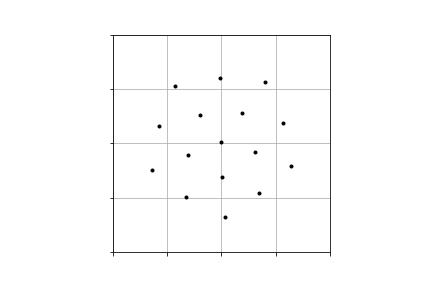
\includegraphics[width=0.7\columnwidth,height=60mm,keepaspectratio]{../figures/cover_photo.png}
   \vfill
   \setlength{\tabcolsep}{0pt}

   \begin{tabular}{p{40mm}p{\dimexpr\columnwidth-40mm}}
                   Project Title: & \textbf{Machine Learning for Communications with Short Block Length} \\[12pt]
                   Student: & \textbf{Alistair P. S. Wallace} \\[12pt]
                   CID: & \textbf{01062642} \\[12pt]
                   Course: & \textbf{EEE4} \\[12pt]
                   Project Supervisor: & \textbf{Dr Bruno Clerckx} \\[12pt]
                   Project Cosupervisor: & \textbf{Dr Morteza Varasteh} \\[12pt]
                   Second Marker: & \textbf{Dr Cong Ling} \\
   \end{tabular}
\end{titlepage}

%%%%%%%%% Contents Page

\section*{MUST DO BEFORE SUBMISSION}

\begin{itemize}
   \item Correct Figure 1b Block, Diagram.
   \begin{itemize}
      \item Transmitter and Receiver the wrong way round.
      \item Receiver spelt "Reveiver"
   \end{itemize} 
   \item Find bug or remove all caps section about unfound bug in BPSK encoding section.
   \item Got through and find all typos
   \item Remove pseudo code snippets, not necessary.
\end{itemize}


%%%%%%%%% ABSTRACT
\begin{abstract}   
   This report focused on applying recent developments in machine learning to the field of communications to improve performance over channels which are unknown or difficult to model. It has been shown that optimising each stage of a communication system individually gives suboptimal performance, leading to investigating end-to-end learnt communication systems, where the optimal communication system can be learnt for a particular channel, environment and for specific hardware non-idealities.
   
   The report reproduces results from two recent papers ~\cite{oShea,Aoudia} on the subject, exploring unsupervised models and investigating supervised models with additive white Gaussian noise (AWGN), Rayleigh block fading (RBF). It then goes further by applying the above methods to Ricean fading (RF) channels.
   
   The report produced predominantly similar results to ~\cite{oShea} for supervised models, giving identical performance for two of the three ($n$,$k$) configurations. However, differences were found, sometimes showing lower performance of the technology in question or less aesthetic t-distributed stochastic neighbour embedding (t-SNE) based constellation diagrams, which the original authors overlooked.
\end{abstract}
\pagebreak

\section*{Acknowledgements}
This project is the culmination of not only my work, but also the help given by others. I would like to thank my supervisor Bruno Clerckx for his advice, supervision and feedback on the written sections of the report. Secondly I would like to thank 
my co-supervisor Morteza Varasteh for always being reachable for assistance, for his help with the implementation of the project and for helping me understand the underlying fundamentals of communication.

\pagebreak


\tableofcontents
\pagebreak

\FloatBarrier
\section{Introduction}

\subsection{Introduction to the subject}

This project is on machine learning for communications with short block lengths. A typical communication system is shown in Figure \ref{fig:ClassicalCommsBlockDiagram}. As can be seen, it has many discrete modular parts, all of which are optimised individually, however, it has been shown that this gives sub-optimal performance~\cite{ChannelEncodingOptimality}.

\begin{figure*}[t!]
   \centering
   \begin{subfigure}[t]{0.45\textwidth}
      \centering
      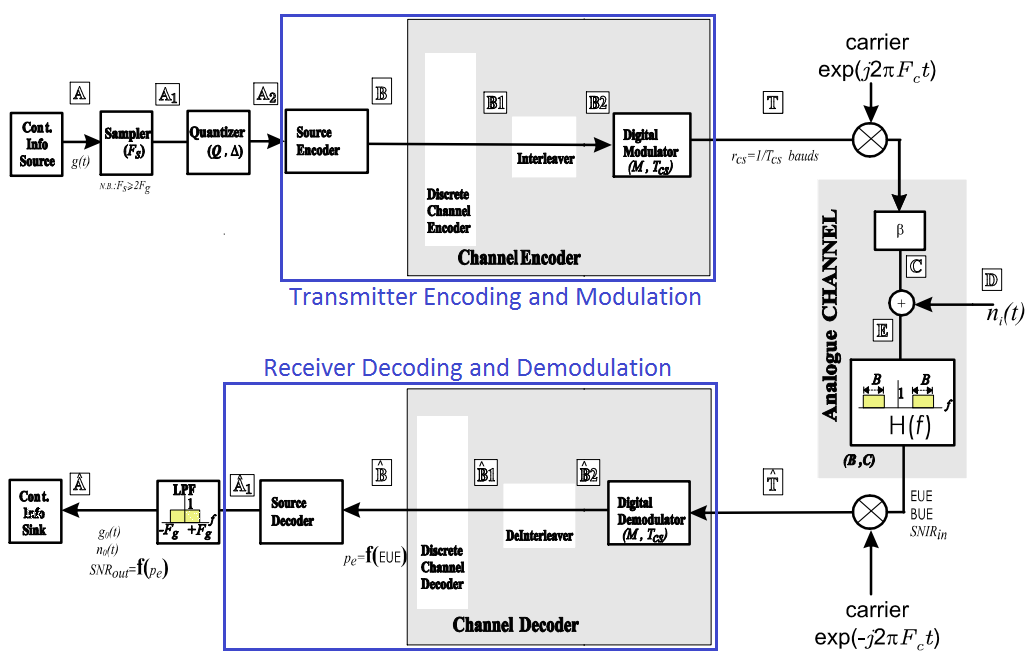
\includegraphics[width=\linewidth]{figures/classical_comms_block_diagram.png}
      \caption{A block diagram of a classical communications system. Taken from ~\cite{EE3CommsSystemsNotesL4}.}
      \label{fig:ClassicalCommsBlockDiagram}
  \end{subfigure}
  ~
  \begin{subfigure}[t]{0.45\textwidth}
       \centering
       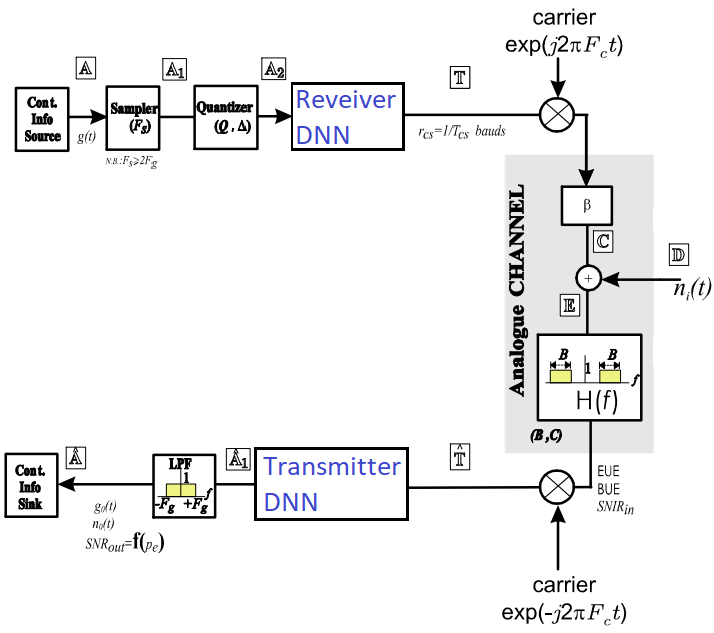
\includegraphics[width=\linewidth]{figures/dnn_block_diagram.png}
       \caption{A block diagram of a DNN based communication system. Based on a diagram from ~\cite{EE3CommsSystemsNotesL4}.}
       \label{fig:DNNCommsBlockDiagram}
   \end{subfigure}
   \caption{A comparison of a classical and DNN based architecture to show how the DNNs simplify the architecture.}
   \label{fig:tSneConstellationDiags}
\end{figure*}


The idea of this research is to replace all the individually optimised modules with one deep neural network (DNN) each for the transmitter and receiver. This involves replacing everything within each blue box in Figure \ref{fig:ClassicalCommsBlockDiagram} with one neural network (NN), as is shown in Figure \ref{fig:DNNCommsBlockDiagram}. 

Normally the information goes through two sets of encoding, source encoding to compress the information content, followed by channel encoding to make it robust to channel noise. Whereas using the DNN method all of the communication system's encoding can be learned simultaneously, and the overall communication system can be optimised for hardware non-idealities such as non-linear power amplifiers. It also allows the locally optimal communication system for a given channel to be learnt, without trying to categorise or make assumptions about the channel.

\subsection{Project deliverables}

The main aim of this project is to reproduce the results from two recent papers ~\cite{oShea,Aoudia} on the subject. The secondary deliverable was a potential extra objective for if the project was finished early. This deliverable was left unspecified, but would be to do something new. For instance tackling the limitation of being limited to short block lengths, or investigating potential opportunities such as learning an optimal communication system for a channel which could not be mathematically modelled, or could be modelled but couldn't be solved.

The two papers originally contributed five deliverables, four from the first and one from the second. However the project supervisor advised that only the first deliverable from each paper were important and so only these deliverables were attempted. 

The first paper, by O'Shea \etal~\cite{oShea}, was only the second paper on the subject, following a paper 8 months earlier by one of the same authors~\cite{oShea0}. The O'Shea paper first demonstrated that an end-to-end communication system could be learned in an autoencoder like method, the structure of which can be seen in Figure \ref{fig:oSheaAutoencoderLayout}. 

It trained a range of autoencoders across a range of ($n$,$k$) combinations for which the constellation diagrams and performance over different signal to noise ratios (SNRs). These autoencoders had several different types of regularisations which affected their constellation diagrams. Their performance was compared to non-learned methods of encoding, such as BPSK and QAM for channel encoding and Hamming maximum likelihood and hard decision for source encoding. 

\subsubsection{Side note on autoencoders}

Note that while this would be better suited to the background section, it is necessary for understanding the introduction, so it has been placed here.

Autoencoders are a technique used in deep learning (DL) for encoding and compressing data. There are two NNs placed end-to-end, as in Figure \ref{fig:oSheaAutoencoderLayout}. The input to the first network is $s \in \mathcal{M} = \{1,2,\dots,M\}$, where each $s$ can be represented by $k$ bits. The encoder (first network, analogous to the transmitter), compresses $s$ to $x \in \mathcal{N} = \{1,2,\dots,N\}$, represented by $n$ bits. The decoder (second network, analogous to the receiver) decodes $x$ back to $\hat{s}$.

Normally with autoencoders $n < k$, because the autoencoder is finding a compressed form of $\mathcal{M}$ which maintains the information content, while reducing the number of bits used. However in this paper because there is noise added in middle layer, as shown in Figure \ref{fig:oSheaAutoencoderLayout}, $n \geq k$ to increase robustness of the transmitted signal to noise (minimise information loss).

\subsubsection{Project deliverables continued}
\label{sec:deliverables}

Moving back to the O'Shea paper, it should be noted that all the following deliverables were written off by the project supervisor and so were not attempted, they are just described to give a better understanding of the O'Shea paper. 

The paper then went on to investigate training two adversarial networks, but then showed that this was the same as optimising one multiple input multiple output (MIMO) NN with one common or multiple individual performance metrics. Thirdly the authors introduced radio transformer networks (RTNs) which improved performance of the learned communication system in all cases. Lastly the authors investigated using NNs for modulation classification. All of these sections were competitive with or outperformed current state of the art. 


\begin{figure}[t]
   \centering
   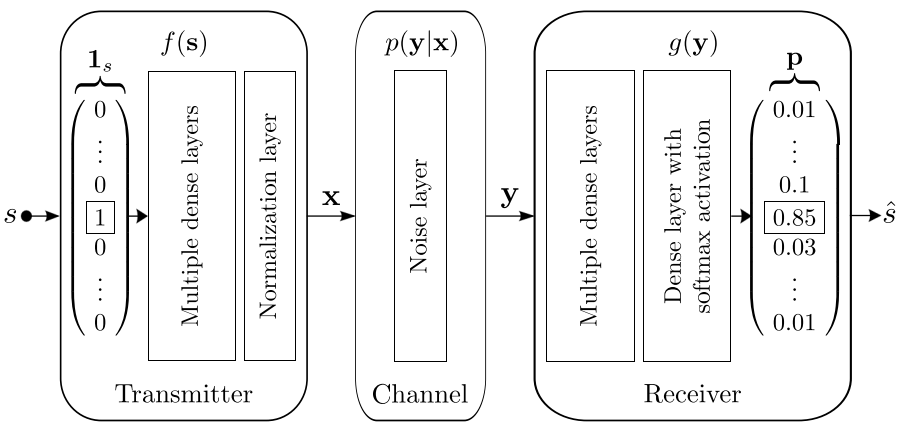
\includegraphics[width=\genfigsize\linewidth]{figures/oShea_autoencoder_layout.PNG}
   \caption{A diagram of the structure of the autoencoder model. Taken from~\cite{oShea}}
   \label{fig:oSheaAutoencoderLayout}
\end{figure}

The details of what the paper achieved will be covered in more detail in the background section, however a high level description was needed as reproducing these results were the main deliverables. Each of these sections would require writing some python code and then using this to reproduce the graphs and constellation diagrams. The authors stated that Keras "has become our primary tool used to generate the numerical results for this manuscript"~\cite{oShea}. Consequently Keras has also been used here to reproduce the results.

The second paper by Aoudia and Hoydis improves on the first by removing the need for a differentiable model of the channel. This helps access the technologies' main potential, which is learning general and optimal communication systems for unmodelable or analytically insoluble channels. 

This paper exclusively solved the problem of implementing reinforcement learning to avoid the need for a differentiable channel model. However it should be noted that supervisor advice says this method's implementation is much more difficult and should not be underestimated.

The main twp deliverables are summarised below.

\begin{enumerate}
   \item Make an autoencoder model and compare it's performance to differential binary phase shift key (DBPSK) and Hamming encoding across a range of signal to noise ratios (SNRs)
   \begin{itemize}
      \item Produce complex channel symbolled (2,2) and (8,8) autoencoders, then obtain their constellation diagrams.
      \item Produce non-complex channel symbolled (7,4) autoencoder and obtain a t-SNE dimensionally reduced constellation diagram.
      \item Write encoding and decoding functions for Hamming HD and MLD
      \item Write encoding and decoding functions for BPSK
      \item Compare the performance of various encoding methods and debug until Figures 3a,b from ~\cite{oShea} were reproduced.
   \end{itemize}
   \item Reproduce the unsupervised reinforcement learning model from ~\cite{Aoudia} which uses the alternate training method. The compare the performance of this model against current state of the art and the autoencoder method across a range of SNRs for an AWGN and an RBF channel.
   \begin{itemize}
      \item Produce a custom layer to implement RBF.
      \item Replicate the paper's supervised model for an RBF channel.
      \item Compare AWGN model from previous deliverable's performance across range of SNRs to the results from the paper. Next do the same with new supervised RBF model.
      \item Produce unsupervised model for AWGN channel
      \item Compare performance of AWGN unsupervised model across range of SNRs.
      \item Produce unsupervised model for RBF channel
      \item Compare performance of RBF unsupervised model across range of SNRs.
      \item Once satisfied all four models are performing as they are reported to have in the paper, assess speed of convergence to correct model for all four AWGN, RBF, supervised and unsupervised models.
   \end{itemize}
\end{enumerate}

Any additional work is likely to fall into one of two categories. Either continueing work on focussed solely on information transfer as in the two main papers ~\cite{oShea,Aoudia}. This would focus on a goal like improving on the work done with reinforcement learning in~\cite{Aoudia}, either tackle the limitations on block lengths, try to improve the convergence time, investigate the systems performance difficult channels or integrating RTNs with the reinforcement learning, as this always improved the results in~\cite{oShea}.

The other option would be to be working on simultaneous wireless information and power transfer (SWIPT) systems. Either investigating the effect of block length on rate-power (RP), obtaining a model that features the practical limitations of the rectenna (rectifier-antenna) used in the EH part, or the dependency between delivered power and channel input average input power.

From assessment of the literature it is thought that it would be better to look into extending the work of reinforcement learning paper, because it better unlocks the potential of this technology. However the supervisor of the project informed the author that the he would decide based on which area was developing fastest at the time.  

From a high level, the project is a software project and so the end deliverables will be a series of python scripts and functions which can learn a full end-to-end communication system. Along side these will be documentation of how to use these functions and scripts as well as comparison of the results produced with the results in the paper's the author is reproducing.

There may be customisations which allow it to use optimal formats for different channels, however this detracts slightly from the idea of an adaptable communication system that can learn an optimal communication system for any long term stationary channel.

Because of the nature of the project there will not be any hardware produced, although there will be some analytical work in analysis of channels.

\subsection{Motivation}

Two reasons for looking into this subject are, the recentness of it's discovery, and the exceedingly promising results, both within the field of communications and of the underlying technology. These within field results are particularly impressive in the long established field of communications where the improvements have become more marginal in modern times~\cite{oShea}.

Other than the intellectual elegance of a fully learned communication system, there are significant advantages to a fully learned system. 

The first reason is that although for known, ideal, mathematically model-able channels there are often mathematically proven optimal methods, (particularly for linear, stationary Gaussian channels), in reality there are many imperfections and non-linearities~\cite{NonLinearities} both in the channel and also in the hardware such as non-linear power amplifiers and finite resolution quantisation. These often cannot be fully accounted for in an analytical solution, leading to sub-optimal performance. Whereas, a fully learned communication system could self-optimise for different hardware configurations and channel environments, with no assumptions about those factors other than stationarity.

Secondly communication systems are normally split into blocks (eg quantisation, modulation, source and channel encoding as shown in Figure \ref{fig:oSheaAutoencoderLayout}). It has been shown that optimising these blocks individually leads to sub-optimal performance, as is shown for the cases of short block lengths and in use on practical channels in ~\cite{ChannelEncodingOptimality, NonOptimalRayleigh} respectively.

A third reason to use NNs is that there have been impressive demonstrations of the learning ability of both feedforward and recurrent NNs (RNNs), suggesting these potentialy promising techniques should be applied to the field of communications. Recurrent NNs have been shown to be Turing-complete~\cite{RnnTuringComplete} and more recently there has been some very impressive work done on learning algorithms with RNNs~\cite{NeuralProgramInterpreters}. 

More relevantly but less recently, feedforward NNs have been shown to be universal function approximaters~\cite{NnUniversalApproximators}. This means that in the limits of width and depth they can approximate any function, even the long and complicated functions of transmitters and receivers.

The combination of these three demonstrations means that a NN should be able to learn any encoding function or algorithm which is optimal, in the limits of width, depth and time. Therefore if the current state of the art methods are really optimal for a given channel, then the NN should converge to these methods, when trained on this channel.

Fourthly due to their inherently parallel nature, NNs are more efficient than most applications at utilising parallel architectures such as GPUs and FPGAs~\cite{FpgaGpuBetterUtilisation}. NNs have also been shown to be very energy efficient with a very high throughput. This higher computations per watt is why Apple are trying to use their neural engine for more tasks in the iPhone~\cite{WiredAppleNeuralEngine}, and is also why it could be suitable to internet of things (IoT) applications.

Additionally it has been shown that NNs maintain high performance at lower precision ~\cite{NnLowFp}, which when combined with their parallel nature can lead to impressively high throughput and low power consumption. This could make this method useful for mobile phone communications because of their limited power budgets and high data needs.

This advantage could be further leveraged by using a chip designed specifically for NNs. This gave ~\cite{Eyeriss} impressively low power consumption. Other specialised chips such as Graphcore's the intelligence processing unit (IPU) claim significant performance increases on graphical processing units (GPUs), often as large as one or two factors of ten higher. A more moderate and already proved example is \cite{GpuIncreasedThroughput} using a GPU to train a network 70 times faster than a single core CPU.

\FloatBarrier
\section{Background}

Due to the novelty of this subject there are a limited number of papers, with the first being from July 2017. Consequently most initial effort was focused on reading and understanding the following three papers ~\cite{oShea, Clerkx, Aoudia}, as well as learning background communications theory from a textbook~\cite{WirelessTextbookC2}. However further but less thorough analysis has been done on a large number of other papers, which are referenced throughout this report. 

A general background will be given on the technology area, before specific sections going into the required deeper detail for the papers which are being reproduced and the elements of communication theory which must be understood.

\subsection{General background}

The first end-to-end learned communications system was from O'Shea \etal ~\cite{oShea,oShea0}. However machine learning had been applied to many jobs within receivers prior to this. Many of these applications such as ``channel identification and equalization, coding and decoding, vector quantization, image processing, nonlinear filtering, spread spectrum applications" and cognitive radios have been summarised in ~\cite{AppsOfNnToComms, AppsNnToCognitiveRadios}. However research supports ~\cite{oShea}'s claim that none of these methods had significant commercial success or adoption.

There has been a sharp rise in the number of applications of NNs to communications, probably largely due to the massive increase in access to open source machine learning libraries such as Tensorflow, Keras and Theano. This has been aided by the impressive and well publicised DL based improvements in computer vision. From this there has naturally been increased research into whether these benefits could be applied to the field of communications.

Applying DL to communications has been approached in two distinct ways. One way is that researchers have tried to apply DL to communications is by improving current algorithms and methods using DL the other is directly replacing the systems. 

Some examples of the first group are improving belief propagation of code words with both feed forward~\cite{AppsNnBeliefPropogation} and recurrent neural networks~\cite{AppsRnnBeliefPropogation}. With the RNN version giving significantly lower complexity whilst maintaining performance. Another example was that applying DL to MIMO detection gave "state of the art accuracy with significantly lower complexity" in ~\cite{AppsNnDeepMimoDetection}. The previous three examples all built on the novel work of ~\cite{AppsNnDeepUnfolding} in applying expert knowledge to NNs.

The second approach, of incorporating DL into communications by replacing the existing methods is the more relevant segment to this report. Initial research into the area was kick-started by a group of papers published during 2016-2017. One example is ~\cite{AppsMimoBlindDetection}, where a sequence of pilot bits were sent across the unknown channel during training to build a non-linear channel model. ~\cite{AppsMolecularComms} applied DNNs to molecular communication where the channel model cannot be modelled mathematically and ~\cite{AppsResourceAllocation} used a DNN to model resource allocation for wireless communication as an unknown linear function, giving "orders of magnitude" speed up compared to state of the art optimisation algorithms.

There has also been some initial research into end-to-end learned communication systems in ~\cite{oShea,oShea0}, with further development of a novel algorithm which uses reinforcement learning to avoid needing a channel model in ~\cite{Aoudia}. Deep learning has also been applied to channel decoding ~\cite{AppsDlChannelDecoding}, radio basis functions ~\cite{AppsRadioBasisFunctions} and improving efficiency in radio transmissions ~\cite{AppsCnnRadioEfficiency}.

\subsection{Paper 1 - An introduction to deep learning for the physical layer}

The first paper released on this subject was by O'Shea and Hoydis~\cite{oShea}, in July of 2017. The paper cites that as communications is quite an established field, so improvements have become more marginal and semi-optimal solutions have been found for most problems. Consequently, a deep learning model (DLM) would have to do very well in order to be of any use. 

DLM’s have historically had a lot of success in fields such as image processing, where it is very difficult to write and algorithm which recognises or does something, but easy for a DLM. Whereas in communications rigid, mathematically backed algorithms for encoding and decoding signals can often be written, so DLMs have never been needed.

First O'Shea and Hoydis demonstrated it was possible to learn a full end-to-end communication system (transmitter, channel and reciever), for a given channel model which is optimised for a chosen loss function, in this case BLER (Block Error Rate). The structure of this model was similar to an autoencoder, however with a noise layer in the middle. The encoder acted as the transmitter, the decoder as the receiver and the noise layer as the channel.

The autoencoder based model was competitive with or outperformed state of the art, in this case Hamming MLD (maximum likelihood decoding), DBPSK, TS-QAM (time sharing quadrature amplitude modulation) and boosted trees. It also offered the potential of being applied to channels which were differentiable, but where the optimal solutions were not known. 

\begin{figure}[t]
   \centering
   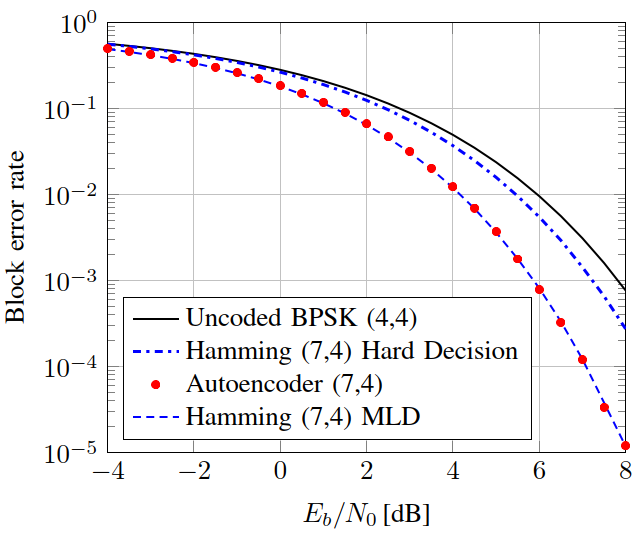
\includegraphics[width=\genfigsize\linewidth]{figures/oShea_autoencoder_hamming_comp.PNG}
   \caption{Comparing block error rate for different SNRs of a learned autoencoder model with current state of the art, Hamming MLD. Taken from~\cite{oShea}}
   \label{fig:oSheaAutoencoderHamming}
\end{figure}

O'Shea and Hoydis then extended this to an adversarial network of many Rx Tx pairs competing for capacity. Next showing this was the same as a single larger MIMO NN which could be optimised in one go with a common or individual performance metric. The jointly learned metric outperformed a TS-QAM system across a range of SNRs as can be seen in \ref{fig:oSheaAutoencoderTsQam}.

\begin{figure}[t]
   \centering
   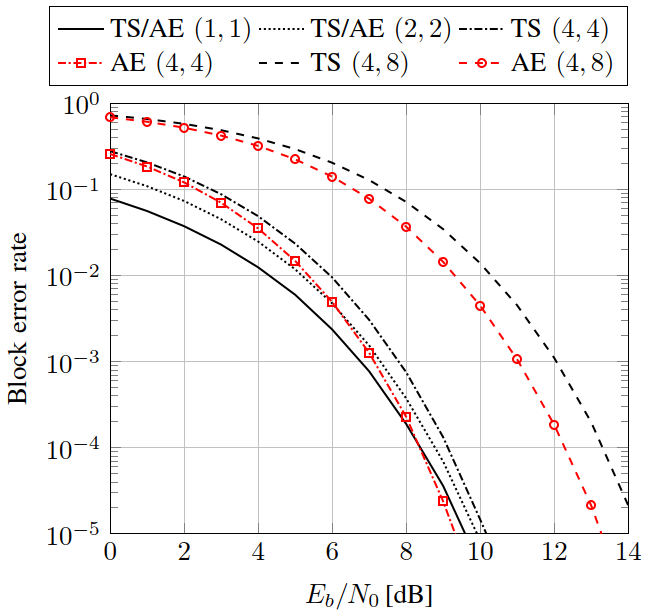
\includegraphics[width=\genfigsize\linewidth]{figures/oShea_autoencoder_TS_QAM.PNG}
   \caption{Comparing block error rate for different SNRs of a learned autoencoder model with a TS-QAM system for a multi-agent communication system. From~\cite{oShea}}
\label{fig:oSheaAutoencoderTsQam}
\end{figure}

It should be noted though that autoencoders perform notoriously poorly with messages they haven't seen before, consequently they normally have to be trained using all the messages from the set of symbols $M = {1,...,M}$. This stops the method scaling to longer block lengths as there are $2^k$ possible messages in a block of lengths $k$ bits. This scaling is particularly poor as the models in this paper used one-hot encoded inputs and outputs, meaning there must also be $2^k$ nodes and the input and output of the system.

After this the authors added an RTN (radio transfer network). RTNs can perform a predefined correction algorithm, for example multiply by a complex number or convolute with a vector. This can be used as a way in incorporate some expert features into a learned system. This was integrated into the DLM for the end-to-end training process and consistently outperformed the normal NN. 

The learned system with added RTN's performance over a Rayleigh channel, with 3 ($L = 3$) fading taps, can be seen in Figure \ref{fig:oSheaRtnRayleigh}. It should also be noted that not only did the RTN consistently outperform current state of the art, it also converged significantly faster than the normal autoencoder. This can be seen in Figure 10 of ~\cite{oShea}.

\begin{figure}[t]
   \centering
   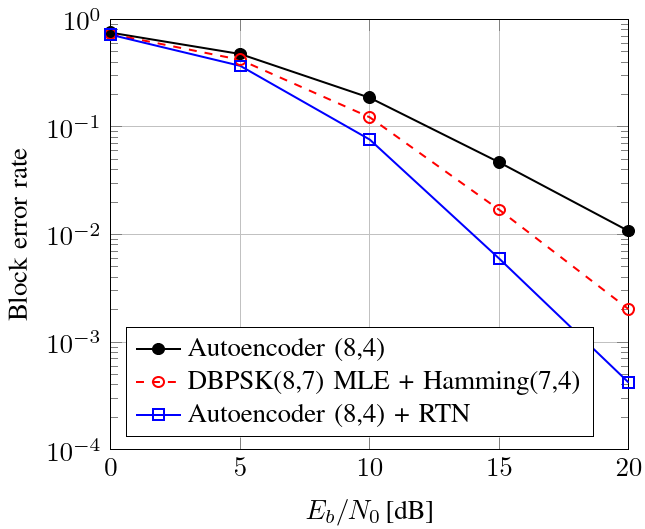
\includegraphics[width=\genfigsize\linewidth]{figures/oShea_autoencoder_RTN_rayleigh_comp.PNG}
   \caption{BLER versus Eb/N0 for various communication schemes over a channel with L = 3 Rayleigh fading taps. Taken from~\cite{oShea}}
\label{fig:oSheaRtnRayleigh}
\end{figure}

Lastly O'Shea and Hoydis used a convolutional neural network (CNN) on raw coplex valued in-phase and quaternary (IQ) samples and found that it outperformed traditional classification techniques using expert features. This is consistent with the current trend that learned features are better than expert ones. 

\begin{figure}[t]
   \centering
   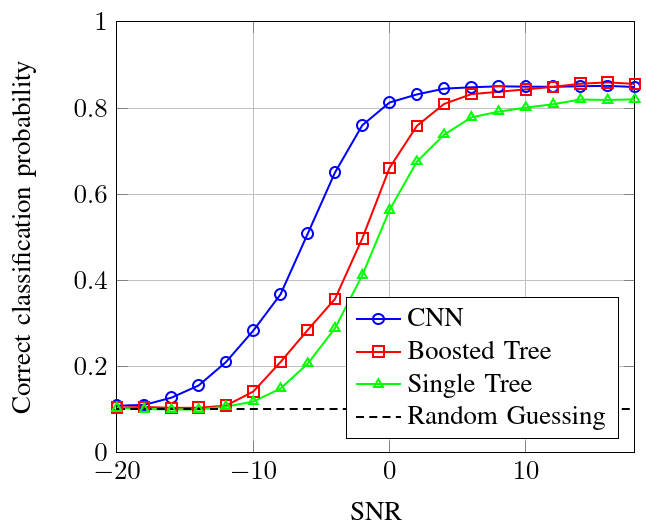
\includegraphics[width=\genfigsize\linewidth]{figures/oShea_CNN_Rx_classification.PNG}
   \caption{Classification performance comparison versus SNR. Taken from~\cite{oShea}}
\label{fig:oSheaCnnRxClassification}
\end{figure}

In conclusion, comparison with traditional baselines showed extremely competitive BLER, however the inherent autoencoder lack of scalability makes this method impossible for any long block length communication. This method also requires a differentiable mathematical model for the channel, which is severely limiting as a big opportunity for this technology would be to learn optimal communication systems for channels we can't model. This was still a very promising area though with potential uses of optical communications, where the channel impairments are highly non-linear and notoriously difficult to model and compensate for. Or alternatively unusual or complicated channels.

\FloatBarrier
\subsection{Paper 2 - End-to-end learning of communication systems without a channel model}

As highlighted in the conclusion of the O'Shea paper, if an autoencoder like NN is used to learn a communication system then the channel model must be  differentiable. This paper ~\cite{Aoudia}, written by Aoudia and Hoydis in April 2018, exclusively set out to remove the need for a channel model. 

They produced a novel algorithm which solves the problem by iterating between the supervised training at the receiver and reinforcement learning (RL) at the transmitter. They showed it worked as well as supervised methods using additive white Gaussian noise (AWGN) and using Rayleigh block-fading (RBF) channels. Their method converged slower on AWGN but faster on RBF as can be seen in Figure \ref{fig:AoudiaTrainingSpeeds}. This is the first step towards learning comms systems over any type of channel without any prior assumptions. 

\begin{figure}[t]
   \centering
   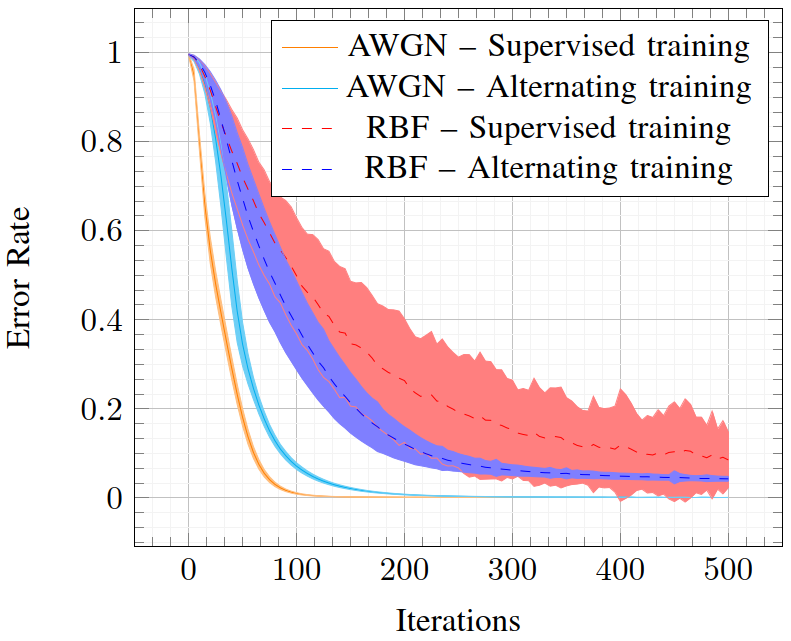
\includegraphics[width=\genfigsize\linewidth]{figures/Aoudia_relative_training_speeds.PNG}
   \caption{Evolution of the error rate over the first 500 iterations. Taken from~\cite{Aoudia}}
\label{fig:AoudiaTrainingSpeeds}
\end{figure}

The reason this innovation was so important is that channels are normally black boxes, where only the inputs and outputs can be observed. The authors used a method called "Policy Learning", which is a subsection of RL. RL provides a theoretical foundation for obtaining an estimate of the gradient of an arbitrary loss function with respect to actions taken by an agent. In this case the agent is the transmitter and loss is performance metric provided by the receiver. This would mean knowledge of the channel model and instantaneous channel transfer function is not needed which allows them to train an autoencoder purely from observations. 

The "alternating training algorithm" trains the receiver first then the transmitter, alternating between training each side while keeping the parameters for the other side fixed. The receiver is trained using mini-batch stochastic gradient descent (SGD) as in other methods. For training the transmitter a random perturbation vector $\mathbf{w}$ is added. This is done for a whole batch of transmitted messages, these messages are then sent across the channel, and received as normal, the losses are calculated, and then transmitted back to the transmitter along a lossless channel. Finally a normal optimisation step is done using SGD where the loss-gradient is estimated using Equation 4 from ~\cite{Aoudia}. 

The authors found that the alternating method took longer to converge with for the AWGN channel but less time for the RBF channel than the supervised learning method. However it had the same end performance as the supervised method in both cases. This performance can be seen in Figures \ref{fig:AoudiaPerformanceAwgn} and \ref{fig:AoudiaPerformanceRbf}.

\begin{figure}[t]
   \centering
   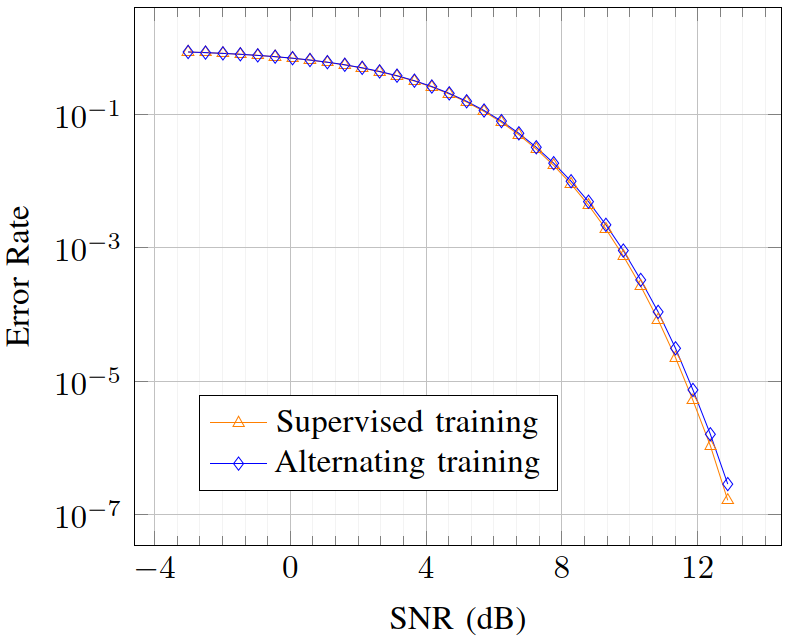
\includegraphics[width=\genfigsize\linewidth]{figures/Aoudia_AWGN_performance.PNG}
   \caption{Alternative training vs autoencoder methods for AWGN Channel. Taken from~\cite{Aoudia}}
\label{fig:AoudiaPerformanceAwgn}
\end{figure}

\begin{figure}[t]
   \centering
   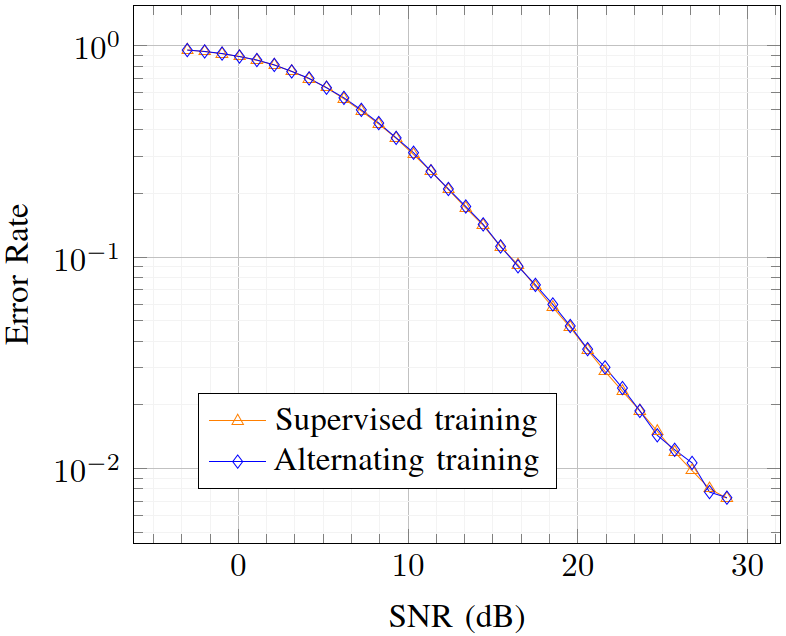
\includegraphics[width=\genfigsize\linewidth]{figures/Aoudia_RBF_performance.PNG}
   \caption{Alternative training vs autoencoder methods for RBF Channel. Taken from~\cite{Aoudia}}
\label{fig:AoudiaPerformanceRbf}
\end{figure}

In conclusion Aoudia and Hoydis showed that they could achieve the same end performance to a fully supervised approach, but without needing a mathematical model of the channel, so it could therefore be applied to any type of channel without prior analysis. 
Although their algorithm currently requires an additional reliable channel during training to feedback losses from the receiver to the transmitter, this is still a huge step. It also does not solve help the problem of being restricted to short block lengths, and arguably makes it worse in the case of AWGN as the method takes longer to converge even with shorter block lengths. Lastly it should also be noted that the networks for the AWGN and RBF channels are not actually the same and the RBF network's structure incorporates expert knowledge of the channel. So this method is not as general as it first seems.

However the importance of this step should not be underestimated. It allows learned communication systems to be used on channels which are either unknown, or too complex to model, which is arguably the biggest potential benefit of this technology. 

\FloatBarrier
\subsection{Paper 3 - A learning approach to wireless information and power transfer signal and system design}

This paper, written by Varasteh, Piovano and Clerkx has a slightly different focus. The previous two papers focused solely on achieving reliable communications with low error rates, this paper focuses on simultaneous wireless information and power transfer (SWIPT) using a nonlinear model, an autoencoder. This paper on learned SWIPT systems is motivated by the fact that designing SWIPT signals and systems analytically is very cumbersome. 

There is a fundamental trade-off between the information rate and the power rate and so the NNs are optimised using a joint loss function. The observed results were inline with previously known theoretical results, particularly in that as you raise the demand for energy, the constellation diagram converges to one point a long way out along one of the axes, and the others closely clustering around the origin. However while this is what they would expect from the theory, it would not be possible to find these results theoretically or using numerical methods. So these found constellation, which can be found in Figure \ref{fig:VarastehConstellationDiagrams}, diagrams are novel and significant.

\begin{figure}[t]
   \centering
   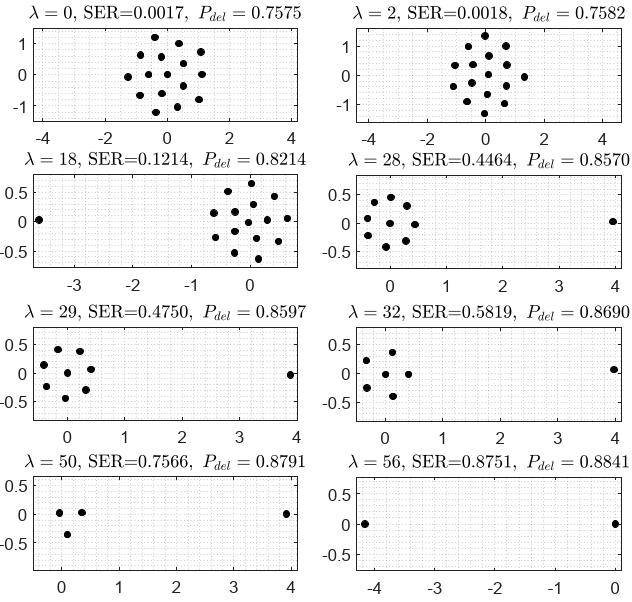
\includegraphics[width=\genfigsize\linewidth]{figures/Varasteh_novel_constellation_diagrams.PNG}
   \caption{Representation of 16-symbols modulation for different values of λ (different information rate and power demand at the receiver) with SNR 20 dB. By increasing λ, the delivered power at the receiver increases. Taken from~\cite{Clerkx}}
\label{fig:VarastehConstellationDiagrams}
\end{figure}

To have good SWIPT it is essential to model the energy harvester (EH) with a high level of accuracy, which is an antenna and a rectifier with fundamentally non-linear characteristics. In the literature it is usually modelled linearly, however using an NN allows it to be modelled non-linearly. Interestingly if you model the EH  linearly an analytical study found it prefers single carrier transmissions and also there is no trade-off between information and power transfer.  Whereas non-linear models favour multi-carrier transmission and have a trade-off between the two objectives.

The results were promising, the autoencoders and surpassed the performance of state-of-the-art algorithms. The more channel symbols, the more DC power is received by the receiver. This is because to optimally transmit lots of power the transmitter favours the high probability information symbols around zero, and the low probability information symbols a long way from zero along on of the two axes. The more symbols you have the better it can fit the ideal pdf with all but one clustered symmetrically around the origin.

The symbols near the origin are called the information symbols, and the one far away from the origin is referred to as the power symbol. Additionally the authors found that as the power demand increases, more of the channel symbols are sacrificed to increase the power delivery. Normally by mapping more of the information symbols to the origin. 

Another interesting observation by the authors was that the delivered power was "directly dependent on the channel input average power constraint". This means that two systems trained at the same SNR but with different transmitted powers would have different designs. However they left investigation of this aspect to another paper, along with investigation of the effect of block lengths on delivered power and making a model that features practical limitations of the rectenna non-linearity accurately.

In conclusion, this paper had some significant and completely new results, for instance the constellation diagrams would be impossible to find analytically because of the computational complexity of finding them. But in this paper they were able to find them using machine learning.

\subsection{Background communications theory}

\subsubsection{Types of fading}

Fading can be categorised into large or small scale, fast or slow and flat or frequency selective. Large scale fading is is due to path loss of signal as a function of distance and shadowing by large objects, such as buildings and hills. Because of it's large spacial size it is usually frequency independent. Small scale fading is due to constructive and destructive interference of multiple signal paths between the transmitter and the receiver. This smaller spacial scale is of the order of the carrier wavelength and is therefore a function of frequency. 

In a learned communication system these factors could be taken account of, and as long as they were stationary an optimal communication system could be learned with no assumptions. Taking advantage of these factors is something a traditional communication would find more difficult.

\begin{figure}[t]
   \centering
   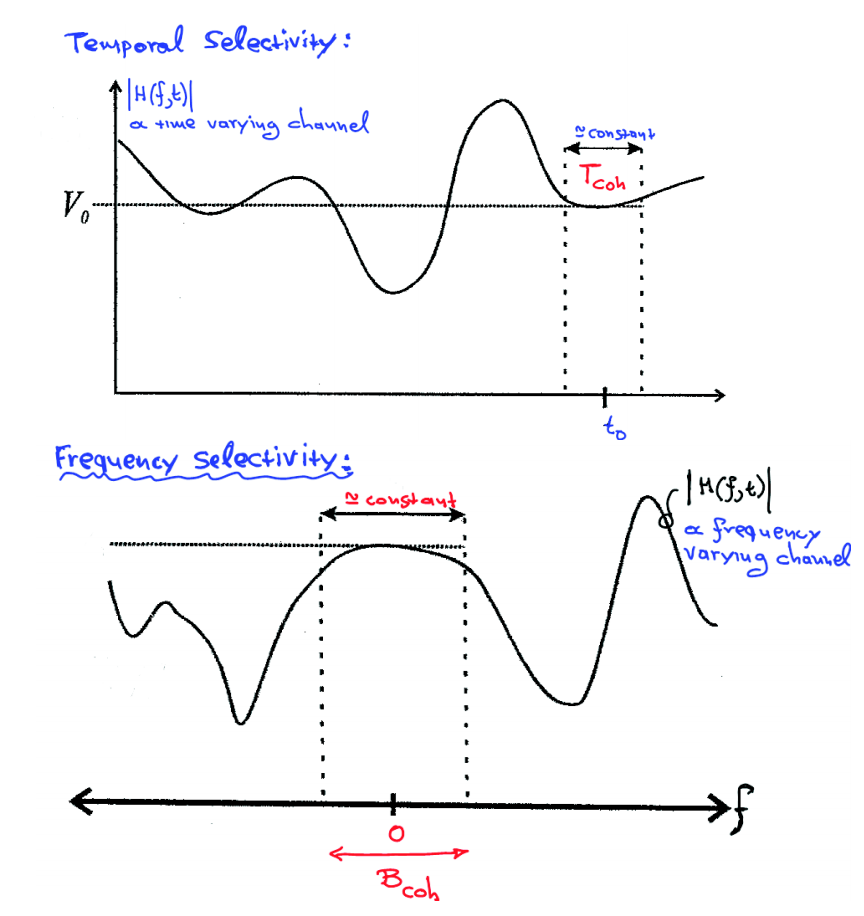
\includegraphics[width=\genfigsize\linewidth]{figures/time_freq_coherence.PNG}
   \caption{A figure to demonstrate the meaning of coherence time ($T_{coh}$) and coherence bandwidth ($B_{coh}$) from~\cite{EE3CommsSystemsNotesL4}}
\label{fig:coherence_illus}
\end{figure}

To explain fast and slow fading we must first explain the meaning of coherence time. Coherence time is the time for which a channel is roughly constant as is shown by the diagram in Figure \ref{fig:coherence_illus}. There is little consensus as to exactly what fast and slow fading means~\cite{WirelessTextbookC2}. One interpretation is that a channel is fast fading if the coherence time is less than the delay requirement of the application, whereas is defined as slow fading if the coherence time is greater than the delay requirement of the application. However another definition which is shown in ~\cite{EE3CommsSystemsNotesL4} and is demonstrated in Figure \ref{fig:fast_slow_flat_freq_selec_fading} is that fading is fast if the time per channel symbol ($T_{cs}$) is greater than the coherence time ($T_{coh}$).

\begin{figure}[t]
   \centering
   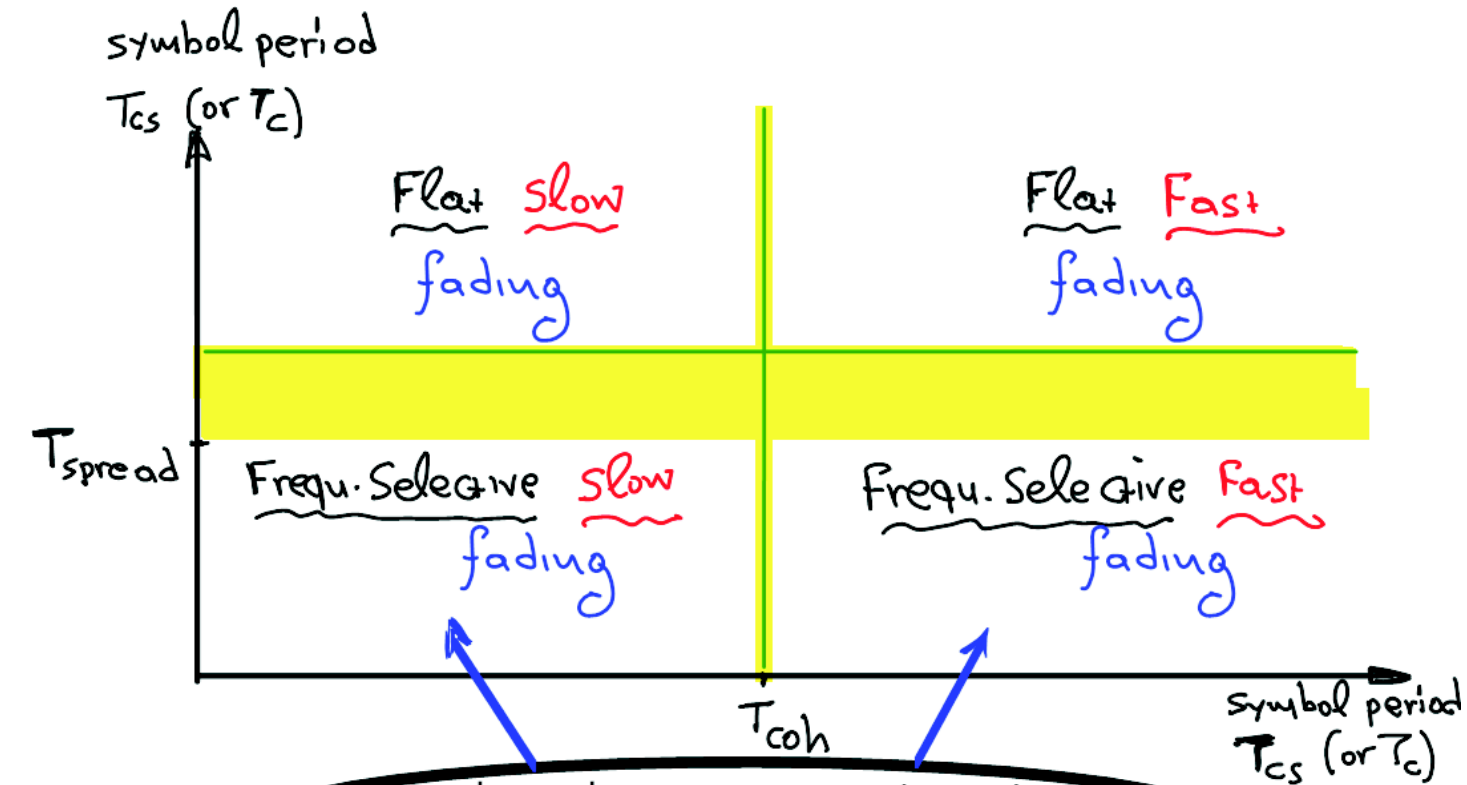
\includegraphics[width=\genfigsize\linewidth]{figures/fast_slow_flat_freq_selec_fading.PNG}
   \caption{A figure showing how to classify a channel as fast/slow and flat/frequency selective fading taken from~\cite{EE3CommsSystemsNotesL4}}
\label{fig:fast_slow_flat_freq_selec_fading}
\end{figure}

Defined either way the main difference between the two is that in fast fading channels you can transmit channel symbols over multiple channel fades, whereas in a slow fading channel you must transmit over that particular fade. This is either to satisfy the delay requirement of the application, or because your $T_{cs}$ is much shorter than your $T_{coh}$. Note that this behaviour depends on the channel characteristics (affects $T_{coh}$), the frequency (affects $T_{cs}$) and the application (sets the delay requirement). For instance voice transmission usually has quite a low delay requirement of ${\sim}100$ms~\cite{WirelessTextbookC2}, but in different channels and transmitting at different frequencies could be either slow or fast fading.

Flat and frequency selective fading are similarly defined as can be seen in Figure \ref{fig:coherence_illus}. Fading is flat if $T_{cs}$ is greater than $T_{spread}$. This means that the multi-paths for consecutive channel symbols will not overlap. Frequency selective fading is where the $T_{cs}$ is less than $T_{spread}$ and so multi-paths for consecutive channel symbols will overlap.

Faster, flatter fading is easier to design a communication system for. In the cases of frequency selective fading, which through the multi-paths depends on the environment, a learned communication system could learn an optimal system. This is another case of something which might be much more difficult to do analytically.

Because of these characteristics it seems likely that a learned communication system would be more suited to a very complex, but stationary environment. A good example of this may be an urban environment with many multi-paths. This would be very hard to model analytically and to do so would likely require assumptions which might make the solution sub-optimal. Whereas a learned system would avoid all these assumptions and learn the local optimum for that environment. However note that an urban environment may be too non-stationary for this method to work.

\subsubsection{Capacity and block lengths}

Shannon's capacity formula (Equation \ref{eqn:ShannonAwgnCapacity} taken from~\cite{WirelessTextbookC5}) describes a theoretical limit on the capacity of an AWGN channel as a function of SNR, however it does not specify a method of achieving said bound.

\begin{align}
    C_{AWGN} &= B.\log_2(1 + \frac{P}{\sigma^2})  \mbox{    (bits/sec)} \nonumber\\
    C_{AWGN} &= \frac{1}{2} \log_2(1 + \frac{P}{\sigma^2})  \mbox{    (bits/symbol)}
    \label{eqn:ShannonAwgnCapacity}
\end{align}

AWGN channels are now normally decoded using iterative decoding algorithms which are far faster but have very similar performance to maximum likelihood decoders, such as "turbo" and "low density parity check" (LDPC) codes~\cite{WirelessTextbookC5}. Using LDPC codes much lower error probabilities can be achieved by using longer block lengths~\cite{WirelessTextbookC5} to approach maximum theoretical capacity.

Another driver towards long block lengths is that Shannon's separation theorem proves, that if you separate the source encoding and the channel encoding, then this approach becomes theoretically optimal in the limit of infinitely long block lengths~\cite{ChannelEncodingOptimality}. This has led to most communication being done over very long block lengths. In OFDM if the block length is already very long then coding jointly across sub-carriers cannot increase the rate of reliable communication~\cite{WirelessTextbookC5}.

Capacity in fading channels must be thought of in a different way because whatever code is used the bit error probability ($p_e$) cannot be made arbitrarily small because the probability that the channel is in deep fade is non-zero~\cite{WirelessTextbookC5}. Deep fade is strong destructive interference which can result in temporary failure of communications due to a massive drop in channel SNR, so will cause an error whether the signal is encoded or not. It should also be noted that Equation \ref{eqn:FadingVsAwgnCapacity} always holds.

\begin{equation}
    C_{Fading} \leq C_{AWGN}
    \label{eqn:FadingVsAwgnCapacity}
\end{equation}

Because the probability of deep fade is non zero the strict sense capacity is zero. instead we find $C_{\epsilon}$ where $P(deep fade) < \epsilon$. However despite the fact we think about it differently the conclusion is the same for fast fading (time varying) channels. Because the code-words span several coherence periods the outage probability improves. This is because you can treat the different coherence periods as independent identically distributed (i.i.d) variables. By the law of large numbers their total variance will be lower. Extending this principle we like the block lengths to be long both to average out the effects of the Gaussian noise and the fluctuations of the channel. Hence the same conclusion, long block lengths.

Unfortunately using long block lengths has downsides. Firstly long block lengths give significant coding delays increasing latency even though they maintain throughput. Because of this in applications with tight delay constraints you may still get outage. Secondly for cases common in IoT applications where not much data needs to be send, long block lengths are not necessary and are impractical. 

Note that the gains in longer block lengths are not as big for slower fading channels, so potentially this could be an area which a learned network of short block length communications systems could do well.

A problem with this environment though is that communication systems in slow fading channels often use feedback to the receiver to use \textit{channel inversion} to increase their capacity. Channel inversion is where the transmitter varies the input power to keep the receiver SNR constant~\cite{WirelessTextbookC5}. This can consume huge amounts of power though and so is not appropriate for IoT applications. So, if the learned communication system could be adaptable or had a mechanism for feedback from the receiver to the transmitter then it might provide an alternative to channel inversion. Making communication in slow fading channels much more possible for IoT applications.

For all of these cases above where long block lengths are not feasible, short block lengths are necessary. However the coding techniques used for long block lengths have been shown to be sub-optimal~\cite{ShortBlockLengthNonOptimality} when used with short block lengths. Because of this there is a motivation to learn communications techniques specifically for this area.

\subsection{Additional notes}

This technique has great potential for providing flexible communication across highly non-linear, unmodelable or mathematically insoluble channels. However it should be noted that in the case of non-stationary channels this method does not really have any potential without significant addition. The method could potentially be adapted to become adaptive, however this may be particularly difficult. This is because even in the most advanced form using the reinforcement learning you still require a noiseless channel between the receiver and the transmitter to communicate back what was received. 

This is fine if you are pre-training the network for a stationary channel you can train it with a noiseless channel temporarily. However if you are trying to update the weights online then you may lose significant capacity or use valuable resources such as frequency trying to transmit back the received bits to train the transmitter. This weakness for non-stationary channels is very important as most wireless channels are highly non-stationary. 

\subsection{Analysis of competing products}

The O'Shea paper~\cite{oShea} being replicated claimed there had not been much adoption of ML in commercial use ~\cite{oShea}, which at the time of writing was true, however this has now changed. After some research the main commercial competition found was a start-up called DeepSig. One of it's two co-founders was Tim O'Shea, the co-author of the two founding papers on the subject of end-to-end learned communication systems. It currently has two commercial products OmniSIG and OmniPHY.

OmniSIG is a software package that allows training and monitoring of a communication system on a range of hardware devices. The package claims to often provide a 4-10 dB improvement and 10x reductions in computational complexity ~\cite{DeepsigOmnisig}. OmniPHY seems to be similar system however the information on DeepSig's website is not very informative about what the product does, other than it learns a communication system, much like the OmniSig~\cite{DeepsigOmniphy}. DeepSig appears to be in it's infancy, and the author has been unable to find any other companies which are working in this area, suggesting it is still a very new corporate area. Additionally it is not entirely surprising that DeepSig seems to be the first, as it's founder is one of the founders of the field. 

If this report was producing a commercial application then such intellectually established competition would be quite worrying. So while only producing an academic report is being produced, it makes the research arguably less valuable as there is less chance for a company to get an early monopoly on the market. 

On the subject of competing papers and academics, due to the nature of the project being to reproduce the results of two existing papers, there are by definition competing papers. Alongside the two papers that have been reproduced here ~\cite{oShea,Aoudia} there are also several existing papers which have applied similar methods to similar problems. However few papers have learned a whole end-to-end communication system and the ones that have have been analysed in greater detail above.

\subsection{Analysis of necessary software tools}

One of the project specifications given to the author was to do the project in python and so this is why the python language was chosen. Although given a free choice python would still have been selected due to the large amount of high quality machine learning libraries available in python, such as Keras and Tensorflow. Another reason is that the large python community contributes to faster debugging and more support. Python 3.6.8 is being used because at the date of starting it is the latest version of python that supports Tensorflow and Keras. 

The main software tool that being used is Keras with a Tensorflow backend. These are both open source machine learning libraries designed to make machine learning easier at a higher level. Allowing users to describe complicated networks in many fewer lines of code. The other reason that Keras has been chosed is that the two paper's being reproduced both specify that they used Keras~\cite{oShea,Aoudia}. 

\subsection{Analysis of necessary hardware}
\label{sec:HardwareAnalysis}

The main hardware specification is what device is needed to be able to train and test Keras models on. While any modern cpu core will be able to run Keras, it would be significantly faster to train and test on a graphical processing unit (GPU) as shown here~\cite{TensorflowBenchmarking}. But tensorflow and keras can still run on a simple cpu, and this requirement will be satisfied by any modern laptop or desktop. 

The hardware which has been chosen to use is a HP Spectre with an Intel I7 6500u. This was chosen because of the convenience of it being the author's own laptop. This hardware has been used for the majority of the code development and running. However training of large models or many models has been run on an amazon web services (AWS) g3.4xlarge instance to take advantage of the speed up associated with using a GPU.

A g3.4xlarge is equipped with 16 high frequency Intel Xeon E5-2686 v4 (Broadwell) processors and one NVIDIA Tesla M60 GPU, with 2048 parallel processing cores and 8 GiB of video memory. This significantly increased the speed of training models. This instance was selected because of it's high quality GPU, but also because of the author's familiarity with it from a fourth year course.

\FloatBarrier
\section{Evaluation Strategy}

The two main deliverables are to reproduce the results from two papers ~\cite{oShea,Aoudia} as laid out in Section \ref{sec:deliverables}. Consequently assessing the completeness of the above deliverables should be relatively simple, in that the results produced can be compared with the results that are being reproduced, and if they are the same then the deliverable is complete.

For both papers performance of models was assessed by comparing the results of the code to the graphical results in the paper as there are no numerical results provided. Extra testing and validation was done along the way to check the the models were giving reasonable results. Strategies for this included plotting constellation diagrams, testing the system with no noise and using unit tests for BPSK and Hamming encoding methods.

To ensure written code was correct, code written for previous deliverables was used for testing new code, producing results for learned systems and current state of the art, to give ball park figures to check the code was roughly working. Then each small function was tested thoroughly to ensure the overall system was working. Where it was hard to predict whether the results made sense they were checked against theoretical estimations, and if there was still uncertainty the project supervisors was consulted. 

Some extra comparisons which will be completed if there is time for evaluation of whether the developed methods are truly competitive with state of the art are comparing the learned systems to Shannon's theoretical capacity limit and current state of the art codes such as turbo and LDPC codes for an AWGN channel.

The generality of a particular architecture of learned communication system will be evaluated by comparing the learned networks and current state of the art across common fading channels such as Rayleigh and Ricean channels across a range of type of fading, large scale or small scale, fast or slow, flat or frequency selective. This would better evaluate the generality of a learned communction system than has so far been done in the literature.

This generality could be further evaluated by doing the same for some rare or hard to model channels. These being where the learned communication system should have the biggest advantage and so it would be interesting to see if they could deliver on their potential.


\FloatBarrier
\section{Design and Implementation}

\subsection{Paper 1 - Producing an Autoencoder}

An autoencoder based communication system which could be trained was been produced relatively quickly, however it originally contained a bug causing it to not use all of the possible communication symbols. This was suspected to be due to the regularisation method, however was slow to fix.

\subsubsection{Initial autoencoder model}

The development was started by building a simple autoencoder model in using Keras with a Tensorflow back-end. This was trained on the $M=2$ ($k=1$) case with one hot encoded inputs and outputs. 

The model had a single dense layer transmitter, L2 normalisation layer, a Gaussian channel layer and a single dense layer receiver. This meant when tested after training over 1000 epochs it gave the input output relationship shown in Figure \ref{fig:CodeInitialOutput}.

\begin{figure}[t]
   \centering
   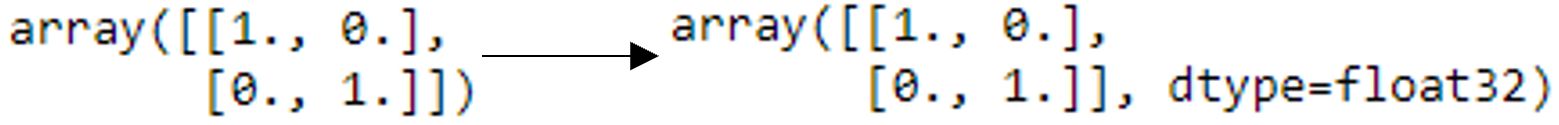
\includegraphics[width=0.8\linewidth]{figures/initial_ae_output.png}
   \caption{The input output of the initial autoencoder model during testing. }
\label{fig:CodeInitialOutput}
\end{figure}

\subsubsection{Adding noise at test time}

Clearly no noise has been added in the testing case. This was because the built in GaussianNoise layer in Keras is a training layer and so does not add noise if not in the training phase. To solve this problem a custom layer was added which adds noise both during training and testing as a channel model should. The code for this layer can be found by searching for "class GaussianNoise" in the \code{initial$\_$dnn$\_$comms.ipynb} notebook from the project github~\cite{AwGithub}. This changed the input output relationship to the one shown in Figure \ref{fig:CodeGaussianNoise2}.

\begin{figure}[t]
   \centering
   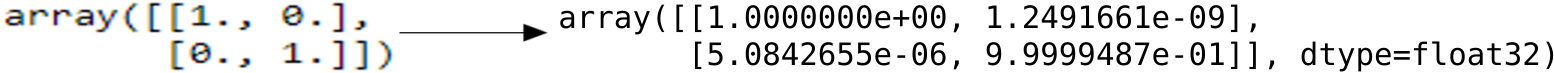
\includegraphics[width=0.8\linewidth]{figures/ae1_1_with_noise.png}
   \caption{The input output of the autoencoder model with gaussian noise added at test time. }
\label{fig:CodeGaussianNoise2}
\end{figure}

\subsubsection{Adding a most likely symbol layer}

The output of the receiver was a softmax layer, which gave an aposteri probability distribution for the sent symbol, given the received signal. However at test time it is desirable to know the bit error rate (BER), which requires discrete bits.

To deal with this another custom layer was added to the output of the model which would take in the aposteri probability distribution and output the most likely symbol. An example of input output of this layer is shown in Figure \ref{fig:MostLikelySymbolLayer}.

\begin{figure}[t]
   \centering
   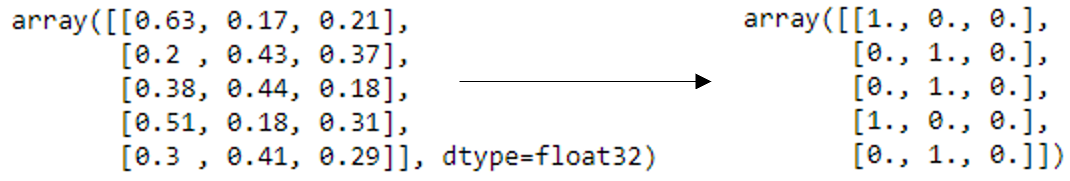
\includegraphics[width=0.8\linewidth]{figures/most_likely_symbol_io.PNG}
   \caption{The input output of the MostLikelySymbol layer for a randomly generated discrete pdf input. }
\label{fig:MostLikelySymbolLayer}
\end{figure}

This layer was originally written using a numpy based function, however this would not compile as part of the Keras model. This was because Keras could not differentiate the layer, which is required when training NNs for back propogation, and so could not train the model. So a custom layer was written using Keras Tensorflow back-end functions which worked.

\subsubsection{Making the channel symbols complex numbers}

Next the channel symbols were turned into complex numbers to represent the in-phase and quaternary sections of the transmitted signal. This required modifying the channel nodes of the model to have an extra dimension, which in turn forced a change in the regularisation layer.

This allowed channel symbols to be meaningfully plotted. Some channel symbols for a (2,2) autoencoder are shown in Figure \ref{fig:WrongConstellationDiagram}, but there are clearly only three constellation points, despite the fact there should be four as it should converge to a QPSK constellation diagram. This was because the model had not learnt the $(1,1)$ channel symbol and so the first and third symbols were mapped to the same channel symbol. This was clearly an error, however it's source was not yet found until later. 

\begin{figure}[t]
   \centering
   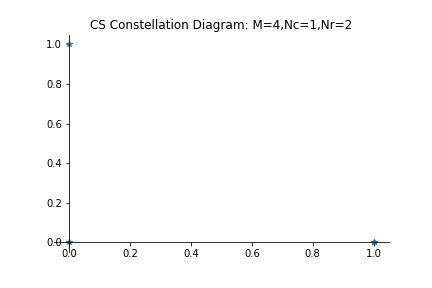
\includegraphics[width=\genfigsize\linewidth]{figures/wrong_constellation_diagram.png}
   \caption{A constellation diagram produced by a trained (2,2) model which was clearly wrong. }
\label{fig:WrongConstellationDiagram}
\end{figure}

\begin{figure}[t]
   \centering
   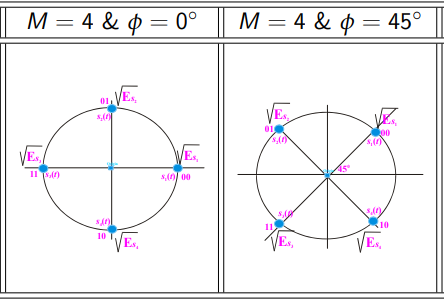
\includegraphics[width=\genfigsize\linewidth]{figures/EE3-03_comms_systems_qpsk_constellation_diagram.PNG}
   \caption{An example of a correct QPSK constellation diagram taken from ~\cite{EE3CommsSystemsNotesL4}. }
\label{fig:CommsSystemsConstelDiagEg}
\end{figure}

Another obvious error from this constellation diagram was that the four points were only mapped to binary x and y coordinates. A normal QPSK constellation diagram would be expected to look more like what is shown in Figure \ref{fig:CommsSystemsConstelDiagEg}. In Figure \ref{fig:CommsSystemsConstelDiagEg} all of the points have an equal magnitude from the origin but are at phases $90^{\circ}$ apart, to maximise separation for a given transmission power. This suggested that there was an error in the regularisation layer, which made this the focus for the next section. 

\subsection{Paper 1 - Producing an Autoencoder}

\subsubsection{Batch vs L2 normalisation}

L2 normalisation and batch normalisation are defined below by Constraint \ref{eq:L2Normalisations} and Equation \ref{eq:BatchNormalisation} respectively:

\begin{subequations}
\begin{align}
   \left[\sum_{i=1}^{n}\left \| x_i \right \|^2\right]^{\frac{1}{2}} &= 1 \label{eq:L2Normalisations}\\
   \mu_B &= \frac{1}{n} \sum_{i=1}^{n}x_i \\
   \sigma_B^2 &= \frac{1}{n} \sum_{i=1}^{n} \left(x_i - \mu_B \right)^2 \\
   y &= \frac{x_i - \mu_B}{\sqrt{\sigma_B^2 + \epsilon}}
   \label{eq:BatchNormalisation}
\end{align}
\end{subequations}

\begin{figure*}[t!]
   \centering
   \begin{subfigure}[t]{0.2\textwidth}
       \centering
       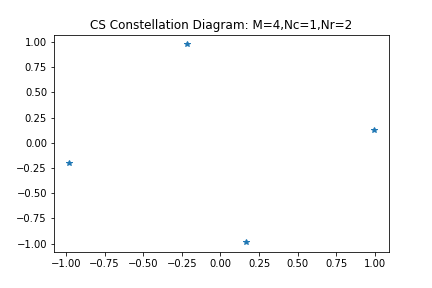
\includegraphics[width=\linewidth]{figures/ae2_2_correctish_relu_const_diag.png}
       \caption{The first batch normalisation model's constellation diagram.}
   \end{subfigure}
   \hfill
   \begin{subfigure}[t]{0.2\textwidth}
       \centering
       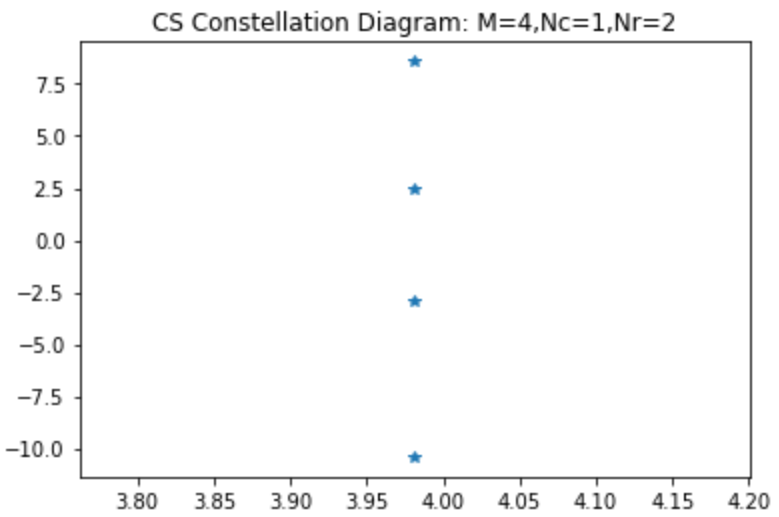
\includegraphics[width=\linewidth]{figures/ae2_2_wrong_const_diag_1d.png}
       \caption{An incorrect constellation diagram where all the points only varied in one dimension, however were not placed on the origin of the other dimension.}
   \end{subfigure}
   \hfill
   \begin{subfigure}[t]{0.2\textwidth}
       \centering
       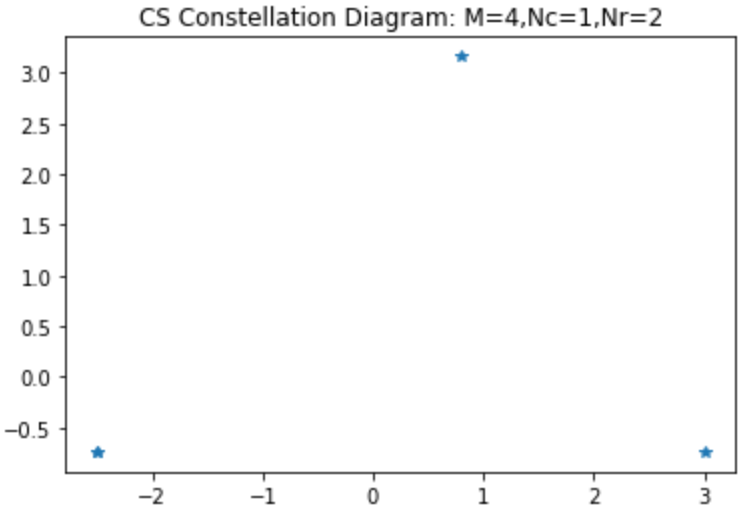
\includegraphics[width=\linewidth]{figures/ae2_2_wrong_const_diag_3points.png}
       \caption{The common convergence to three instead of four channel symbols.}
   \end{subfigure}
   \hfill
   \begin{subfigure}[t]{0.2\textwidth}
       \centering
       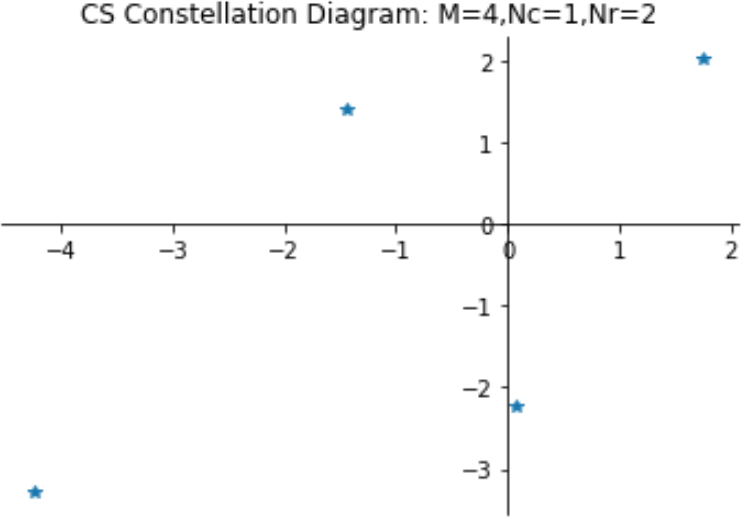
\includegraphics[width=\linewidth]{figures/ae2_2_wrong_qpsk_kite_w_title.png}
       \caption{A more promising constellation diagram, with four points varying in two dimensions, however not in the correct shape.}
   \end{subfigure}
   \caption{Examples of the missleading initial results obtained whilst using batch normalisation.}
   \label{fig:BatchNormConstDiags}
\end{figure*}


Batch normalisation was briefly investigated, and initially gave the promising looking constellation diagram shown in Figure \ref{fig:BatchNormConstDiags}a. This was a vast improvement on the previous constellation diagram shown in Figure \ref{fig:WrongConstellationDiagram}. This motivated further investigation into batch normalisation to try and get the final small changes needed to reproduce QPSK. During this investigation 
the batch size was changed, the data size increased and axis over which BatchRegularization was performed was changed.

However all of these changes resulted in worse constellation diagrams than the original diagram shown in Figure \ref{fig:BatchNormConstDiags}a. Eventually it was found that this diagram was also unreproducible, and this result seemed to have been a missleading fluke caused by the inconsistency of the model's performance from one intialisation to another.

The missleading results were also partially due to a bug, causing of a layer being bypassed. After lots of testing batch normalisation was rejected in favour of the original L2 normalisation, however over a different axis. 

Batch normalisation simulates a unit average power constraint with zero DC component. However to obtain the QPSK constellation a constant instantaneous power constraint was needed, which was emulated by L2 normalisation in the last layer of the transmitter. This means that the L2 normalisation method was more appropriate and reintroduction of the L2 normalisation led to the contellation diagrams in Figure \ref{fig:InconsistentReluConstDiags} being produced. 

These constellation diagrams, while still inconsistent and not always correct, were always varying in two dimensions and had a unit instantaneous power budget so were an improvement on the constellations produced from the batch normalisation.

At this point the style of the constellation diagrams was changed to match the style of those in the paper for easier comparison. The square format made identifying QPSK and 16 QAM constellations simpler.
   
\begin{figure*}[t!]
   \centering
   \begin{subfigure}[t]{0.2\textwidth}
       \centering
       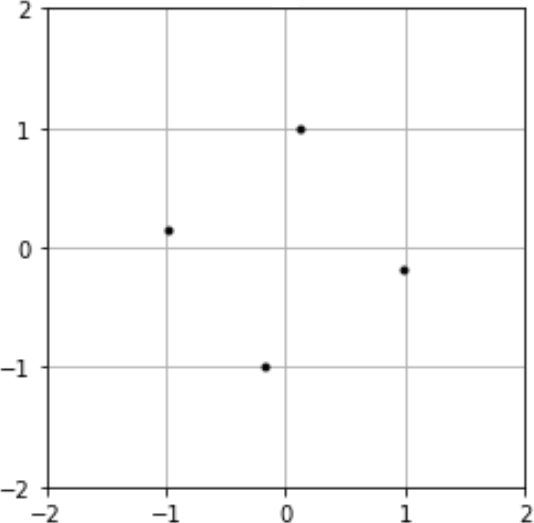
\includegraphics[width=\linewidth]{figures/l2_ae_inconsistent1.png}
       \caption{A correct (2,2) constellation diagram}
   \end{subfigure}
   \hfill
   \begin{subfigure}[t]{0.2\textwidth}
       \centering
       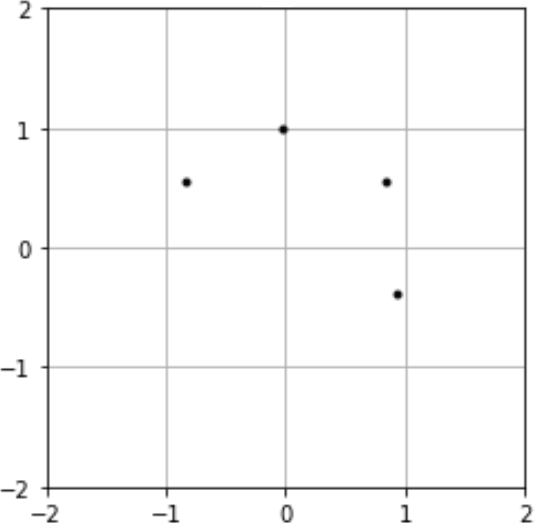
\includegraphics[width=\linewidth]{figures/l2_ae_inconsistent2.png}
       \caption{Incorrect (2,2) constellation diagram}
   \end{subfigure}
   \hfill
   \begin{subfigure}[t]{0.2\textwidth}
       \centering
       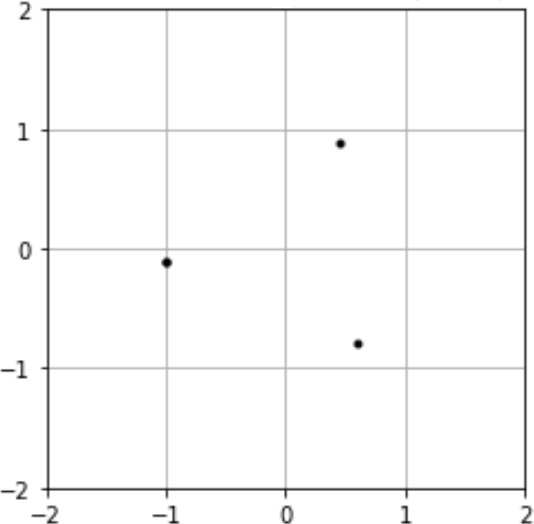
\includegraphics[width=\linewidth]{figures/l2_ae_inconsistent4.png}
       \caption{(2,2) autoencoder convergence to three instead of four channel symbols.}
   \end{subfigure}
   \hfill
   \begin{subfigure}[t]{0.2\textwidth}
       \centering
       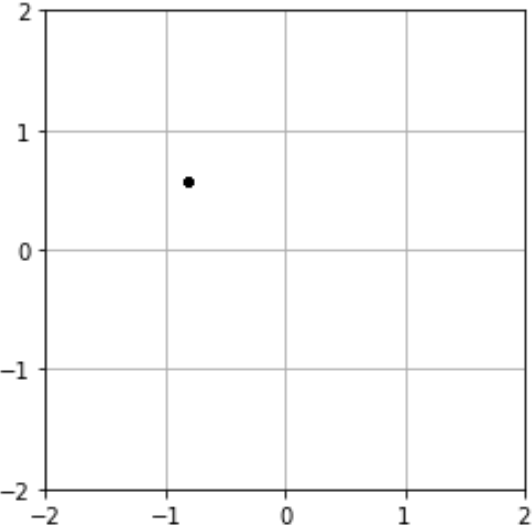
\includegraphics[width=\linewidth]{figures/l2_ae4_2_inconsistent.png}
       \caption{(4,2) autoencoder convergence to one instead of sixteen channel symbols.}
   \end{subfigure}
   \caption{Four example constellation diagrams illustrating the inconsistency of the original L2-normalised (2,2) and (4,2) autoencoders with ReLu activation functions.}
   \label{fig:InconsistentReluConstDiags}
\end{figure*}

\subsubsection{Leaky-Relu over ReLu}

As can be seen in Figure \ref{fig:InconsistentReluConstDiags} the constellation diagrams were not consistent at all. Occasionally, roughly one in ten times, the (2,2) model would converge to the correct QPSK constellation diagram. However often it would either have multiple input points converge to the same channel symbol, or would converge to a diagram which was clearly not optimal.

Meanwhile the (4,2) model was underfitting and consistently converging to one channel symbol instead of sixteen, but the exact channel symbol changed each time. This suggested that the model was underfitting, either due to insufficient layers or an inappropriate activation function.

Some research suggested that both these issues might be to do with "neuron death" giving dependence on initialisation values. This is a problem characteristic of the ReLu activation function, shown in Figure \ref{fig:ReluAndLrActivationFunction}a. The ReLu activation function outputs zero for all non-positive inputs, meaning that if weights are initially set so that a neuron consistently outputs a negative value pre-activation-function, it will consitently output a zero.

\begin{figure*}[t!]
   \centering
   \begin{subfigure}[t]{0.2\textwidth}
       \centering
       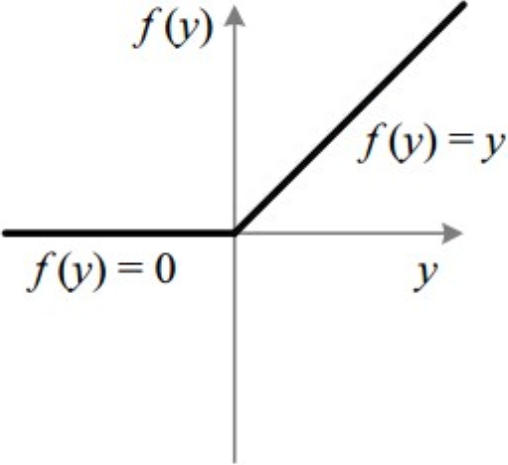
\includegraphics[width=\linewidth]{figures/relu_activation_function.png}
       \caption{ReLu activation function.}
   \end{subfigure}
   ~
   \begin{subfigure}[t]{0.2\textwidth}
       \centering
       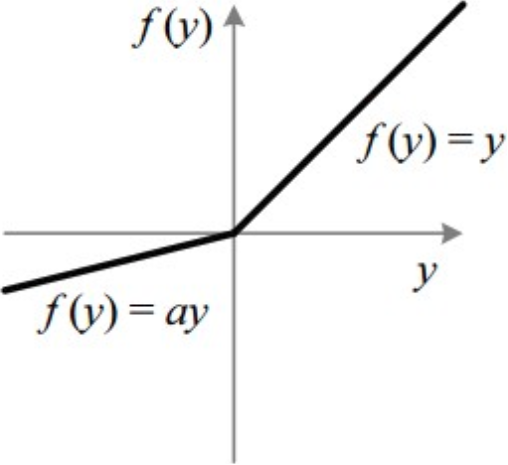
\includegraphics[width=\linewidth]{figures/leaky_relu_activation_function.png}
       \caption{Leaky-ReLu activation function, typically $a\approx0.01$.}
   \end{subfigure}
   \caption{}
   \label{fig:ReluAndLrActivationFunction}
\end{figure*}

This means that the weights will not be updated through back-propogation as the partial derivatives of the error with respect to the weights will be zero. As a result the model will not improve for these neurons and will converge at an incorrect solution. 

A suggested solution to this problem was using a "leaky-relu" activation function, shown in \ref{fig:ReluAndLrActivationFunction}b instead. A brief trial of this showed much improved performance, prompting further investigation into alternative activation functions in the section below. 

The improved (2,2) constellation diagram seen in Figure \ref{fig:Lr22ConstDiags}a was consistently produced with each channel symbol being equally spaced, centred around the origin, having an equal magnitude and a phase difference of $90^{\circ}$ from adjacent points. The only parameter which changed phase of the point in the first quadrant. The (4,2) constellation diagram shown in Figure \ref{fig:Lr22ConstDiags}b was also produced for the first time and was then consistently reproduced. 

\begin{figure}[t]
   \centering
   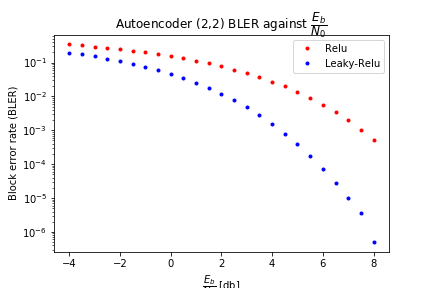
\includegraphics[width=\genfigsize\linewidth]{figures/autoencoder_2_2_bler_EbNo_leaky_vs_relu.png}
   \caption{A comparison of the BLER performance of two leaky-ReLu and ReLu based (2,2) autoencoder models.}
   \label{fig:ReluVsLrBlerAcrossSnrs}
\end{figure}

The BLER of two ReLu and Leaky-ReLu based models were also found over a range of SNRs. This was done to ensure that the metric of test error at training SNR was valid for evaluating model quality. It could be possible that some activation functions performed better at some SNRs and worse at others. The results of this are shown in Figure \ref{fig:ReluVsLrBlerAcrossSnrs}. The leaky-ReLu model consistently outperforms the ReLu model across all $\frac{E_b}{N_0}$ ratios. This both confirms that leaky-ReLu is a better activation function for this problem and that test error at training SNR is a valid metric for assessing model quality.

Now that successful models had been reproduced all of the layers in the models were named so that the weights could be saved and loaded into new models to avoid the time overhead of retraining larger models. The model weights were saved in the \code{.h5} format because neither the JSON nor YAML formats worked with the custom \code{GaussianNoise} and \code{MostLikelySymbol} layers.

\begin{figure}[t]
   \centering
   \begin{subfigure}[t]{0.4\textwidth}
       \centering
       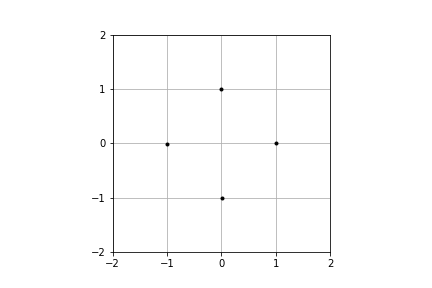
\includegraphics[width=\linewidth]{figures/leaky_relu_qpsk_constellation_diagram.png}
       \caption{QPSK constellation diagram produced by the (2,2) model with a leaky-relu activation function.}
   \end{subfigure}
   ~
   \begin{subfigure}[t]{0.4\textwidth}
       \centering
       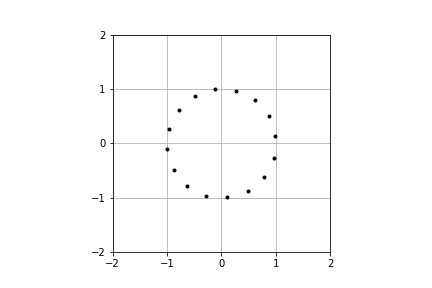
\includegraphics[width=\linewidth]{figures/leaky_relu_16_QAM_constellation_diagram.png}
       \caption{16 QAM constellation diagram produced by the (4,2) model with a leaky-relu activation function.}
   \end{subfigure}
   \caption{}
   \label{fig:Lr22ConstDiags}
\end{figure}

\subsubsection{Comparing different activation functions}

Despite having visually reached the correct constellations for the (2,2) and (4,2) models, due to the vast improvements gained in the previous section from changing the activation functions, six different activation functions were compared in this section.

The six different activation functions were \code{ReLu}, \code{tanh}, \code{sigmoid}, \code{linear}, \code{softmax} and \code{leaky-ReLu}. Because the largest issue faced so far had been lack of consistency, ten (2,2) models were trained for each activation function to assess the consistency of the activation function's performance. Each model was trained for five epochs, over a dataset of $10^7$ shuffled copies of the four possible one-hot-encoded inputs, with a batch size of 4000. At the end of the training, each model was tested on a seperate test set. It's block error rate, constellation diagram and model weights were then all saved before moving onto the next model.

The results can be seen in Figure \ref{fig:ActivationFuncComparison} and Table \ref{tab:ActivationFuncComparison}. It was decided that \code{leaky-ReLu} had marginally outperformed \code{tanh}. This was because, although they had the same average error and same variance of error, leaky-ReLu had a slightly lower minimum value. As the models were only trained for five epochs and as producing the final model would involve selecting the best model over a number of initialisations, it was decided that the minimum error was the most important statistic. Hence \code{leaky-ReLu} was selected as the best activation function. Because of this it was decided to use \code{leaky-ReLu} for all hidden layers, and use \code{tanh} for the output layer to capture non-linearity. 

\begin{table}[H]
\begin{center}
\begin{tabular}{|l|c|c|c|}
\hline
Activation Function & Mean & Min & $\sigma$\\
\hline\hline
ReLu & $0.55835$ & $0.05784$ & $2.30e-1$ \\
Tanh & $0.00156$ & $0.00151$ & $3.00e-5$ \\
Sigmoid & $0.29459$ & $0.29413$ & $3.20e-4$\\
Linear & $0.00157$ & $0.00153$ & $4.00e-5$\\
Softmax & $0.43870$ & $0.29450$ & $9.42e-2$\\
Leaky ReLu & $0.00156$ & $0.00147$ & $3.00e-5$\\
\hline
\end{tabular}
\end{center}
\caption{Activation function performance statistics from ten initialisations}
\label{tab:ActivationFuncComparison}
\end{table}



\begin{figure}[t]
   \centering
   \begin{subfigure}[t]{0.4\textwidth}
       \centering
       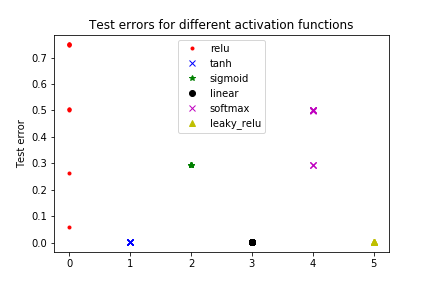
\includegraphics[width=\linewidth]{figures/first_act_f_comparisson.png}
       \caption{Linear axes}
   \end{subfigure}
   ~
   \begin{subfigure}[t]{0.4\textwidth}
       \centering
       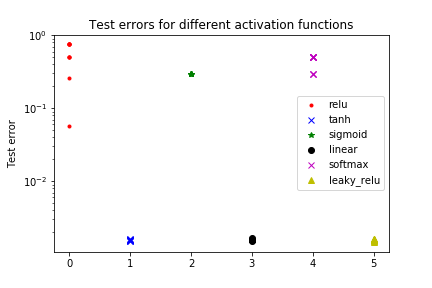
\includegraphics[width=\linewidth]{figures/first_act_f_comparisson_logy.png}
       \caption{Linear x-axis, logarithmic y-axis}
   \end{subfigure}
   \caption{Comparison of the performance of five different activation functions over ten instances of a (2,2) autoencoder model.}
   \label{fig:ActivationFuncComparison}
\end{figure}

\subsubsection{Model training methods}

A number of methods were used during the training of the models to improve the performance of the end model. Firstly it was found that increasing the batch size during training improved the end validation loss. This is supported by the findings of~\cite{IncBatchSize}, which suggest that increasing the batch size is in practice equivalent to decaying the learning rate. The batch size was started at the relatively large batch size of 1000. This lowest point is still relatively large as the noise is randomly generated for each message which is transmitted. Hence the batch size of 1000 is chosen to reduce the dependence on individual noise. This is by the law of large numbers illustrated in Equations \ref{eq:LawLargeNumbers} as a reminder.

\begin{align}
   \mbox{if: } y &= \frac{x_1 + x_2 +\dots + x_n}{n} \nonumber\\
   \mbox{then }  \mathop{\mathbb{E}}[y] &= \mathop{\mathbb{E}}[x] \nonumber\\
   \mbox{and } Var(y) &= \frac{\sigma_x}{\sqrt{n}}
   \label{eq:LawLargeNumbers}
\end{align}

Hence as the batch size is increased the variance of the batch's noise decreases with $\sqrt{\mbox{Batch Size}}$. It is theorised that the model should converge faster if trained at a higher noise variance with a larger batch size, due to the higher noise variance giving larger loss gradients, and the larger batch size smoothing out the gradients to give an equally stationary loss surface. However this has not been tested empirically.

In practice the batch size was varied in three steps, $1000$, $\sqrt{M}*1000$, $M*1000$. It was found that initial progress was made more quickly at a batch size of 1000, because there were more weight updates per epoch, then after the model performance converged at this batch size the batch size was increased and this process repeated twice more. After the batch size was increased each time the performance would at first improve quickly for a few epochs, before slowing and eventually congerging again.

Another method used during the training of the models was to use the EarlyStopping callback in Keras. This was used to try and bring a constant process to training method. The EarlyStopping callback monitored the validation loss and would stop training if the validation loss did not improve after 20 epochs. This method works if the model is being trained over a large number of epochs like 1000, howver not if the model is being trained over 30 epochs. It also has the dissadvantage that it is not stopping at the best model, it is stopping 20 epochs later, so if the validation loss significantly increases due to overfitting in these final 20 epochs then the quality of the end model will be significantly affected. However having a patience parameter of 20 also has the advantage that it can cope with longer flat sections of the loss surface. This has proved useful quite a few times during the training of the larger models, when the validation loss has hardly improved for 20 epochs, before dropping off again more steeply. 

After moving on to reproducing~\cite{Aoudia} the ModelCheckpoint callback was introduced. This would save the model after every epoch, if and only if the validation loss had improved from the current best. This was a better way of ensuring the best model was saved and allowed the patience parameter of the EarlyStopping callback to be increased to improve it's ability to deal with small gradients and flat sections of the loss function.

Training multiple many models with different initialisations should have been used for final models, however due to the consistency of the \code{leaky-ReLu} and \code{tanh} activation functions shown in Table \ref{tab:ActivationFuncComparison} this was not done for the majority of models, however may be used for getting the last few $\%$ of performance out of the final models.  

\subsection{Adding non learned encoding}

\subsubsection{Adding BPSK encoding}
\label{sec:AddingBpsk}

\begin{figure}[t]
   \centering
   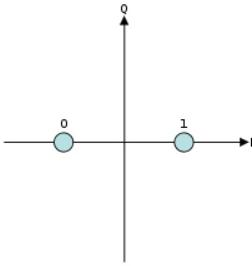
\includegraphics[width=0.2\linewidth]{figures/bpsk_const_diag.jpg}
   \caption{BPSK constellation diagram.}
   \label{fig:BspkConstDiag}
\end{figure}

Binary phase shift keying (BPSK) is the $m = 2$ case of phase shift keying (PSK), also known as 2-PSK. It has two points, seperated by $180^\circ$. It's constellation diagram is shown in Figure \ref{fig:BspkConstDiag}, with two points placed symetrically around the origin on the real axis. It's encoding is given by equation \ref{eq:BpskEncoding}.

\begin{subequations}
\begin{align}
   s_i(t) &= A_c \cos(2\pi ft + \pi(1-i)), \mbox{ i = 0,1} \label{eq:BpskEncoding} \\
   \therefore s_0(t) &= -A_c \\
   \mbox{and } s_1(t) &= A_c
\end{align}
\end{subequations}

Compared to the other m-PSK methods BPSK's channel symbols are the furthest separated and therefore it has the highest tolerance to noise, making it the most robust PSK. This is because it only encodes one bit, so it sacrifices data rate. BPSK's theoretical BER is given by Equation \ref{eq:BpskTheoreticalBer} from~\cite{BpskPe}.

\begin{equation}
   P_b = \frac{1}{2}erfc\left(\sqrt{\frac{E_b}{N_0}}\right)
   \label{eq:BpskTheoreticalBer}
\end{equation}

Where the erfc function is defined by~\cite{ErfcDefinition} as:

\begin{equation}
   erfc = \frac{2}{\sqrt{\pi}}\int_{x=0}^{\infty}e^{-t^2}dt
   \label{eq:ErfcDef}
\end{equation}

The $erfc$ function gives the probability that a $\left| Y \right| \ge x$ where $Y \sim \mathcal{N}(0,\frac{1}{2})$. So $\frac{1}{2}*erfc(x)$ gives the tail probability of a normal distribution ($Y$). 

This relationship means that the theoretical block error rate (BLER) can be calculated to ensure that the experimental graphs found later are correct.

BLER is defined by the European Telecommunication Standards Institue as \textit{"the ratio of blocks received in error to the total number of received blocks, where a block is defined as received in error if the error detection functions in the receiver indicate an error as the result of the Block Check Sequence (BCS)"}~\cite{BlerEtsiDefinition}.

This is taken to mean that if any of the bits in a block are incorrect, then the block is taken as wrong. The BLER is then the percentage of blocks which have any bits which are incorrect. As the noise for each block is assumed to be i.i.d, the above definition gives the following relationship between $P_{be}$ and $P_e$ in Equation \ref{eq:BpskTheoBler}. Note that this assumes stationarity, which is often not a valid assumption in wireless channels.

\begin{align}
   P_{be} &= 1 - (1-p_e)^n \\
   P_{be} &= 1 - \left(1-\frac{1}{2}erfc\left(\sqrt{\frac{E_b}{N_0}}\right)\right)^n
   \label{eq:BpskTheoBler}
\end{align}

\begin{figure}[t]
   \centering
   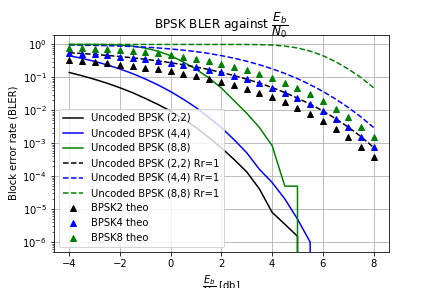
\includegraphics[width=0.6\linewidth]{figures/bpsk_theo_Rr1_and_original.png}
   \caption{BPSK BLER performance over a range of SNRs.}
   \label{fig:BspkBlerComp}
\end{figure}

This theoretical check was actually very useful as it unearthed the second of two bugs in the BPSK encoding and decoding. The graph that made these bugs obvious is shown in Figure \ref{fig:BspkBlerComp}. Stating that results are wrong based on a other results requires a large amount of confidence in the correcting set of results. The theoretical results have this confidence due to matching the values displayed in the paper and the equations producing them being widely agreed upon.

For reference the simulation of the BPSK encoding in the AWGN channel was run by the process outlined in sudo code below. The exact code (which is almost identical) can be found at~\cite{AwGithub}.

\begin{lstlisting}
   # Encode into bpsk
   bpsk_encoded = bpsk_encode_vec(test_data)
   # Add AWGN noise
   noise = std * np.random.randn(bpsk_encoded.shape)
   received = bpsk_encoded + noise
   # Decode from bpsk back to bits
   bpsk_decoded = bpsk_decode_vec(received)
   # Get Block error rate
   return get_block_error_rate(test_data, bpsk_decoded)
\end{lstlisting}

Note that \code{bpsk$\_$encode} and \code{bpsk$\_$decode} were vectorised because it was found that this reduced the latency of the simulation process by approximately $60\%$. This was important, as to give smooth curves the BPSK BLER was tested over a very large test data set and also for 25 different $\frac{E_b}{N_0}$

The first bug was that the noise standard deviation was being calculated incorrectly from the $\frac{E_b}{N_0}$. According to the O'Shea paper the variance is calculated from $\frac{E_b}{N_0}$ using the equation below~\cite{oShea}.

\begin{equation}
   \sigma^2 = \left(2R\frac{E_b}{N_0} \right)^{-1}
   \label{eq:SigmaFromEbN0}
\end{equation}

The paper is not entirely clear with it's definition of $n$, as to whether $n$ is the number of real channel uses or the number of complex channel uses. Originally it was decided the later was correct, meaning that $R = \frac{k}{n_c}$. This was found to be incorrect as it gave incorrect $\sigma$s and this led to if being found that $n$ must be the number of real bits. This gave the change from the solid lines ro the dashed lines in Figure \ref{fig:BspkBlerComp}. The $n_c$ being lower than $n_r$ was making the $R$ two times larger, which was decreasing the variance of the channel noise by a factor of two. This gave the lower error rates shown by the solid lines. The jaggedness of the lines at the lowest error rates was due to insufficiently sized data sets to smoothly represent a error rate in the region of $10^-7$.

At this point the second bug was found.

% NEED TO FIND OUT WHAT IS WRONG WITH MY BPSK ENCODING. I'VE SPENT A WHILE TRYING TO DEBUG IT BUT I CAN'T SEE WHERE I COULD POSSIBLY HAVE AN ERROR, IT IS SUCH A SIMPLE ENCODING AND DECODING METHOD.

After the solving of this second issue the simulated BLER of the BPSK was indistinguishable from the theoretical BLER. Note that all of the code for the BPSK encoding and decoding can be found in the \textit{Implementing Uncoded BPSK} section of \code{initial$\_$dnn$\_$comms.ipynb} at~\cite{AwGithub}.

\subsubsection{Adding hamming hard decision encoding}

Hamming codes are a family of linear block code that allow error detection and correction. They were invented by Richard W. Hamming in 1950, where he laid out the general theory and used the (7,4) as the main example~\cite{HammingOriginalPaper}.

Mathematically there are an infinite number of potential Hamming codes with the following characteristics.

\begin{align}
   r &\geq 2 \\
   \mbox{block length } n &= 2^r - 1 \\
   \mbox{message length } k &= 2^r -r -1
   \label{eq:GeneralHamming}
\end{align}

In the r = 3 case we get the most well known Hamming code, and the one used in this paper, the (7,4) code.

\begin{align}
   r &= 3 \\
   \therefore n &= 2^3 - 1 = 7 \\
   \therefore k &= 2^3 -3 -1 = 4
   \label{eq:Hamming74Characteristics}
\end{align}

In the (7,4) Hamming code, for every four data bits transmitted three parity bits are added. These three parity bits allow the detection and correction of single errors. The combinations of the parity bits are given by Figure \ref{fig:HammingParityVennDiagram} and Table \ref{tab:Hamming74Parity}. Note that the (7,4) Hamming code cannot detect or correct multiple errors. 

However given that the probabilities of one, two and k errors are given by Equation \ref{eq:HammingPe1}, b and d respectively, if $p_e$ is small then the higher order terms will be negligible. For each extra number of errors you become able to correct you will reduce your BER by a factor of $p_e$.

\begin{subequations}
\begin{align}
   p_{e1} &= 1 - \left[(1-p_e)^{4} + 4p_e(1-p_e)^{3} \right] \label{eq:HammingPe1} \\
   p_{e2} &= 1 - \left[ (1-p_e)^{4} + 4p_e(1-p_e)^{3} + 6p_e^2(1-p_e)^{2} \right] \label{eq:HammingPe2} \\
   p_{ek} &= 1 - \left[ \sum_{i=1}^{k}{n \choose i}p_e^i(1-p_e)^{n-i} \right] \\
   \therefore &= \sum_{i=k+1}^{n}{n \choose i}p_e^i(1-p_e)^{n-i}  
   \label{eq:HammingPeN} \\
   \mbox{where: }0 &\leq k \leq n 
\end{align}
\end{subequations}

Hence, despite the fact that the (7,4) Hamming code can only remove single errors this should remove the vast majority of errors and will reduce the BER by approximately a factor of $p_e$, which is likely to be $\approx10^{-3}$.

\begin{table}[H]
   \begin{center}
   \begin{tabular}{|l|c|c|c|c|c|c|c|}
   \hline
   Bit \# & 1 & 2 & 3 & 4 & 5 & 6 & 7 \\
   \hline\hline
   Transmitter Bit & $\mathbf{p_1}$ & $\mathbf{p_2}$ & $\mathbf{d_1}$ & $\mathbf{p_3}$ & $\mathbf{d_2}$ & $\mathbf{d_3}$ & $\mathbf{d_4}$ \\
   \hline
   $\mathbf{p_1}$ & \cellcolor{green}Yes & \cellcolor{red}No & \cellcolor{green}Yes & \cellcolor{red}No & \cellcolor{green}Yes & \cellcolor{red}No & \cellcolor{green}Yes \\
   $\mathbf{p_2}$ & \cellcolor{red}No & \cellcolor{green}Yes & \cellcolor{green}Yes & \cellcolor{red}No & \cellcolor{red}No & \cellcolor{green}Yes & \cellcolor{green}Yes \\
   $\mathbf{p_3}$ & \cellcolor{red}No & \cellcolor{red}No & \cellcolor{red}No & \cellcolor{green}Yes & \cellcolor{green}Yes & \cellcolor{green}Yes & \cellcolor{green}Yes \\
   \hline
   \end{tabular}
   \end{center}
   \caption{A table showing which parity bits interact with which data bits in a (7,4) Hamming code.}
   \label{tab:Hamming74Parity}
   \end{table}
   

\begin{figure}
   \centering
   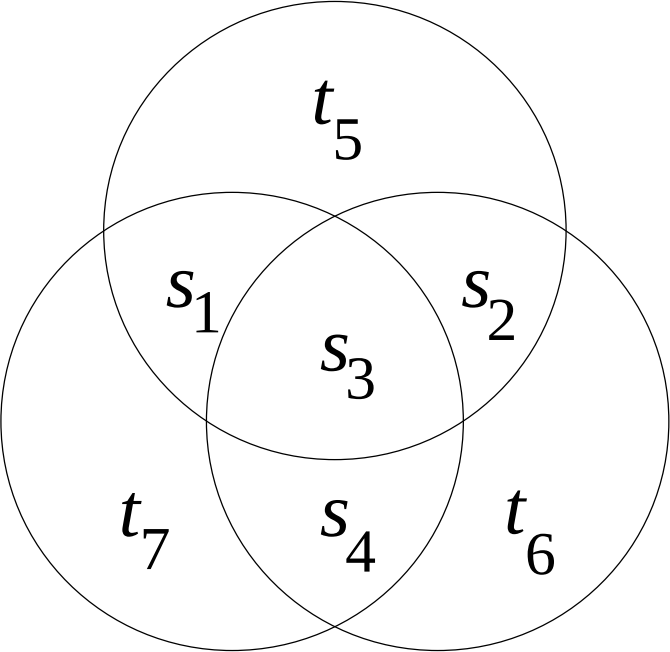
\includegraphics[width=0.2\linewidth]{figures/hamming_parity_venn_diagram.png}
   \caption{Venn diagram showing parity and data bits for a Hamming (7,4) code. Data bits are denoted $s_i$ and parity bits are denoted $t_i$ taken from~\cite{HammingMoonBook}.}
   \label{fig:HammingParityVennDiagram}
\end{figure}

Because the Hamming codes are linear codes, all the encoding and decoding can be performed using linear algebra. To perform the encoding and decoding three matrices are needed. The generator matrix $G$, the parity matrix $H$ and $R$ the decoding matrix~\cite{HammingMoonBook} which are all defined below.

\begin{align}
   \mbox{Generator Matrix: }\mathbf{G} &= \begin{pmatrix}
      1 & 1 & 0 & 1\\ 
      1 & 0 & 1 & 1\\ 
      1 & 0 & 0 & 0\\ 
      0 & 1 & 1 & 1\\ 
      0 & 1 & 0 & 0\\ 
      0 & 0 & 1 & 0\\ 
      0 & 0 & 0 & 1 \\
      \end{pmatrix} \\
   \mbox{Parity Check Matrix: }\mathbf{H} &= \begin{pmatrix}
      1 & 0 & 1 & 0 & 1 & 0 & 1\\ 
      0 & 1 & 1 & 0 & 0 & 1 & 1\\ 
      0 & 0 & 0 & 1 & 1 & 1 & 1
      \end{pmatrix} \\
   \mbox{Decoding Matrix: }\mathbf{R_{ham}} &= \begin{pmatrix}
      0 & 0 & 1 & 0 & 0 & 0 & 0\\ 
      0 & 0 & 0 & 0 & 1 & 0 & 0\\ 
      0 & 0 & 0 & 0 & 0 & 1 & 0\\ 
      0 & 0 & 0 & 0 & 0 & 0 & 1
      \end{pmatrix}
\end{align}

The Hamming encoding step is simple, the transmitter message is produced from the column vector $\mathbf{p}$ by doing the matrix multiplication below in Equation \ref{eq:HammingEncoding}, then taking the second modulus of each element. This is equivalent to taking the last least significant bit of the number in binary. For instance $1 \rightarrow 1$, $2 \rightarrow 0$, $3 \rightarrow 1$.

\begin{equation}
   \mathbf{s} = mod_2(\mathbf{Gp}) = LSB(\mathbf{Gp})
   \label{eq:HammingEncoding}
\end{equation}

The sent message $\mathbf{s}$ then passes through a channel where an error may or may not be added. The received vector is denoted:

\begin{equation}
   \mathbf{r} = \mathbf{s} + \mathbf{e}
\end{equation}

Where $\mathbf{e}$ may be the zero vector. The syndrome vector $\mathbf{z}$ is obtained by matrix multiplying by $\mathbf{H}$. If e has less than or equal to one non-zero element then the result will be H.

\begin{align}
   \mathbf{H_r} &= \mathbf{H}(\mathbf{x} + \mathbf{e}_i) \\
   &= \mathbf{Hx} + \mathbf{He}_i \\
   &= \mathbf{0} + \mathbf{He}_i \\
   &= \mathbf{He}_i \\
   \mathbf{z} &= mod_2\left(\mathbf{Hr}\right)
\end{align}

Noting that $\mathbf{r}$ has been rounded $\mathbf{z}$ is a three bit binary number. If only one bit has been changed then this number corresponds to the index (indexed from one to seven) of the bit which has an error. The value of this bit can be simply flipped to correct the error.

After the error correction stage the message must be decoded. The message is simply recovered my matrix multiplying by $\mathbf{R}$.

\begin{equation}
   \hat{\mathbf{p}} = \mathbf{Rp}
\end{equation}

It should be reiterated that the Hamming (7,4) will incorrectly diagnose multiple bit errors and so will not be able to correct them. As with the previous section the exact code for the Hamming (7,4) Hard Encoding can be found in the \textit{Hamming Hard Decision Encoded BPSK} section of the \code{initial$\_$dnn$\_$comms.ipynb} notebook in ~\cite{AwGithub}, but some psuedo code for end-to-end encoding and decoding process is provided below.

\begin{lstlisting}[escapeinside={(*}{*)}]
   # Encode the one_hot_encoded_vectors into bits
   (*$s$*) = hamming_7_4_encode((*$p$*), G)   
   # Add noise
   (*$e$*) = std * np.random.randn((*$s$*).shape)
   (*$r$*) = (*$s$*) + (*$e$*)
   # Do error correction and decode message
   (*$\hat{p}$*) = hamming_7_4_decode_and_correct((*$r$*), H, R_ham)
   # Get Block error rate
   bler = get_block_error_rate((*$p$*), (*$\hat{p}$*))
\end{lstlisting}

\subsubsection{Initial Hamming HD performance and debugging}

\begin{figure}
   \centering
   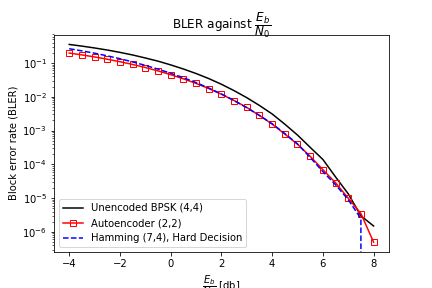
\includegraphics[width=0.6\linewidth]{figures/bler_vs_eb_only_three.png}
   \caption{Original graph of BPSK (4,4), Hamming(7,4) and Autoencoder (2,2) BLER performance, before setting Rr correctly.}
   \label{fig:BlerOriginalHammingBpskAe22}
\end{figure}

After first producing the Hamming (7,4) encoding method it was tested seperately. It was tested using unit several unit test vectors with deterministic errors added. The results of these unit vectors at each stage of the process were compared with results calculated by hand. It was also tested with Gaussian distributed errors added, first with a standard deviation of zero, and then with small standard deviations.

After this seperate training the Hamming (7,4) source encoding was combined with BPSK channel encoding, then it's performance evaluated over a range of SNRs. This performance was then compared to the already produced (2,2) leaky-relu autoencoder model and the BPSK (4,4) model which gave the results shown in Figure \ref{fig:BlerOriginalHammingBpskAe22}


These results did not appear to be correct, despite all three of the encoding schemes having very similar performance across the whole range of SNRs. Thjs aspect was potentially compatible with Figures 3a and 3b because the (2,2) Autoencoder model would be expected to be slightly better than the (4,4) BPSK and slightly worse than the Hamming (7,4) hard decision encoding.

\begin{figure}
   \centering
   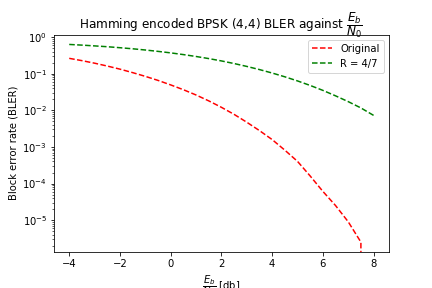
\includegraphics[width=\genfigsize\linewidth]{figures/hamming_correct_Rr_comparison.png}
   \caption{Comparison Hamming HD BLER performance with correct and incorrect values of $R_r$.}
   \label{fig:HammingCorrectRrComp}
\end{figure}

However at $\frac{E_b}{N_0} = 8$ all three of the encoding schemes were achieving BLERs of $10^{-6}$, which was significantly better than the $\approx10^{-3.5}$ results in the paper. The correct relative performance suggested that there was an error with the way the noise variance was being calculated from the $\frac{E_b}{N_0}$.

This intuition was correct, this led to the discovery $n$ being the number of real bits instead of number of complex bits discussed in the Section \ref{sec:AddingBpsk} on adding BPSK. After this error was corrected the Hamming HD BLER performance was a lot more conservative. The difference is shown in Figure \ref{fig:HammingCorrectRrComp}

\subsubsection{Adding Hamming MLD + MLD explanation}

Maximum likelihood decoding is a simple concept. The probability of each possible codeword $s$ in a codebook $s\epsilon S$ having been sent, given a received signal $r$ is calculated. Then the codeword with the maximum likelihood of having been sent is selected. This is mathematically formulated below.

\begin{align}
   \hat{s} &= \underset{i}{\argmax\left[P\left(s_i\;\middle|\;r\right)\right]} \\
    &= \underset{i}{\argmax}\left[\frac{P\left(s_i\cap r\right)}{P\left(r\right)}\right]
\end{align}

Now note that, as this will be computed for all of the possible $s_i$s and the relative size is the only thing which is cared about, the $P\left(r\right)$ can be taken out as a common factor.

\begin{align}
   \therefore \hat{s} &= \underset{i}{\argmax}\left[P\left(s_i\cap r\right)\right] \nonumber
\end{align}

Now given that $s_i$ and $r$ are each made up of $n$ bits, and that as the channel here is AWGN, the noise applied to each bit is treated as independent and identically distributed. Therefore Equation \ref{eq:HammingNoiseIid} is true.

\begin{align}
   P\left(s_i\cap r\right) &= \prod_{j=1}^{n} P\left(s_{i,j}\cap r_j\right)
   \label{eq:HammingNoiseIid}
\end{align}

Now let $n$ be the Gaussian noise vector which is added in the channel. So Equation \ref{eq:HammingPsAndR} can be found from the below equations.

\begin{align}
   r &= s + n \nonumber\\
   \therefore n_j &= r_j - s_{j} \nonumber\\
   \therefore P\left(s_i\cap r\right) &= P\left(N=n_j\right) \nonumber\\
   &= P\left(N=r_j - s_j\right) \nonumber\\
   \mbox{so as: } N \sim \mathcal{N}\left( 0,\sigma^2\right) \nonumber\\
   P\left(s_{i,j}\cap r_j\right) &= \frac{1}{\sqrt{2\pi\sigma^2}}e^{\frac{(r_j - s_{i,j})^2}{2\sigma^2}} \nonumber\\
   \therefore \mbox{ from \ref{eq:HammingNoiseIid}: }P\left(s_i\cap r\right) &= \prod_{j=1}^{n} \frac{1}{\sqrt{2\pi\sigma^2}}e^{\frac{(r_j - s_{i,j})^2}{2\sigma^2}}
   \label{eq:HammingPsAndR}
\end{align}

Therefore the final operator for finding the maximum likelihood estimate of $s$ is given by the two equations summarised below.

\begin{subequations}
\begin{align}
   \hat{s} &= \underset{i}{\argmax}\left[P\left(s_i\cap r\right)\right] \label{eq:HammingFinalSHat}\\
   \mbox{where: } P\left(s_i\cap r\right) &= \prod_{j=1}^{n} \frac{1}{\sqrt{2\pi\sigma^2}}e^{\frac{(r_j - s_{i,j})^2}{2\sigma^2}}
\end{align}
\end{subequations}

To find the maximum likelihood sent message the operator in Equation \ref{eq:HammingFinalSHat} is evaluated on every received codeword. Pseudo code illustrating how the performance of this method was evaluated for a set of messaged denoted $p$ is shown below. The exact code can be found in the \textit{Hamming Encoding with MLD} section of the \code{initial$\_$dnn$\_$comms.ipynb}.

\begin{lstlisting}[escapeinside={(*}{*)}]
   # Encode the one_hot_encoded_vectors into bits
   (*$s$*) = hamming_7_4_encode((*$p$*), G)   
   # Add noise
   (*$n$*) = std * np.random.randn((*$s$*).shape)
   (*$r$*) = (*$s$*) + (*$n$*)
   # Do maximum likelihood decoding
   (*$\hat{s}$*) = ml_decode((*$r$*),bpsk(hamming((*$S$*))),std)
   # Convert ML message out of BPSK
   (*$\hat{p}$*) = bpsk_decode_vec((*$\hat{s}$*))
   # Get Block error rate
   bler = get_block_error_rate((*$p$*), (*$\hat{p}$*))
\end{lstlisting}

Note that the process is made more efficient by entirely skipping the linear algebra of hamming decoding. The bpsk and hamming encoded codewords are used for maximum likelihood decoding instead of the codewords, then the encoded messages are mapped directly back to their original message counterparts using a look-up table. The BPSK decoding step was left in as it was very simple and had been vectorised for numpy making it very efficient already. 

After the Hamming MLD had been implemented it's performance was assessed over a range of SNRs. It performed very well first time, with the only fault being that it was run over too small a data set giving jaggedly lines at low error rates. The performance can be see in Figure \ref{fig:HammingMldBlerAll}.

\begin{figure}
   \centering
   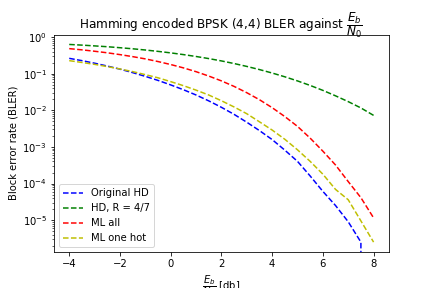
\includegraphics[width=0.6\linewidth]{figures/hamming_7_4_bler_vs_EbNo_comparison.png}
   \caption{Comparison of all Hamming encoding BLERs.}
   \label{fig:HammingMldBlerAll}
\end{figure}

Part of the reason for it's superior performance is that Hamming MLD can correct some multiple bit errors which Hamming HD can not. For instance, in the case where $s = 0,0,0,0,0,0,0$ and $r = 0.5,0.5,0,0,0,0,0$. With Hamming HD the 0.5s would be rounded to 1s, at which point there would be two incorrect bits which could not be decoded by Hamming HD. But in Hamming MLD there is no rounding and this sequence is still closer by Hamming distance to the $s = 0,0,0,0,0,0,0$ codeword than to all other of the codewords.

Out of curiosity the extra performance gain from only transmitting a four bit one-hot encoded vector instead of a a normal four bit vector was investigated. This was interesting because the autoencoders receive $M$ bit one hot encoded vectors instead of $k$ bit normal binary vectors. It was hoped that some parallels might be able to be drawn between the performance gains of the two methods switching between the two. 

The performance of the MLD only transmitting one-hot encoded vectors is shown by Line "\textit{ML half rate}" in Figure \ref{fig:HammingMldBlerAll}. There is a relatively marginal improvement in performance which does not make up for the halfing of the date rate. It should be noted that the autoencoder models are still transmitting the same information content per symbol as the Hamming models they are being compared against as they input a 16 bit one-hot-encoded vector instead of a 4 bit binary encoded vector.

The small improvement in performance suggests that the autoencoder models could likely, given enough training time significantly improve their data throughput by inputting a binary instead of a one-hot-encoded vector, without significantly increasing the BLER.

\subsection{Reproducing Figure 3a and 3b from the O'Shea paper}

\subsubsection{Initial (7,4) autoencoder, t-SNE constellation diagrams and (8,8) autoencoder}

After producing the (4,4) BPSK, (7,4) Hamming HD and autoencoder (2,2) encoding schemes the (7,4) model was produced so that it could be compared against the Hamming HD encoding scheme. This required a different model making function and structure as it could not transmit complex channel symbols. The previous models had transmitted $n_c$ complex channel symbols, however as 7 is an odd number this required a shape of transmitter signals and a new regularisation function. Despite these necessary changes an initial (7,4) model was produced without too many issues. 

The first check on that the autoencoder was performing correctly was to plot the constellation diagram. However this again required a new method. The constellation diagram for the (7,4) model has seven dimensions. So as in the O'Shea paper this was reduced to two dimension using t-SNE. This was done using the \code{sklearn} libraries \code{TSNE} function. 

\begin{figure*}[t!]
   \centering
   \begin{subfigure}[t]{0.3\textwidth}
      \centering
      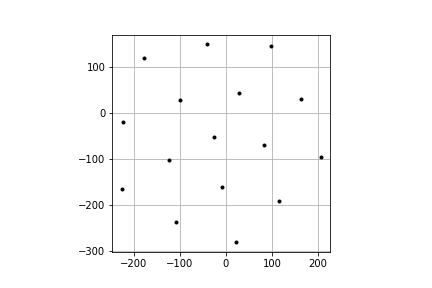
\includegraphics[width=\linewidth]{figures/tSNE_7_4_constellation_diagram_unnormalised.png}
      \caption{Unprocessed t-SNE constellation diagram.}
  \end{subfigure}
  ~
  \begin{subfigure}[t]{0.3\textwidth}
       \centering
       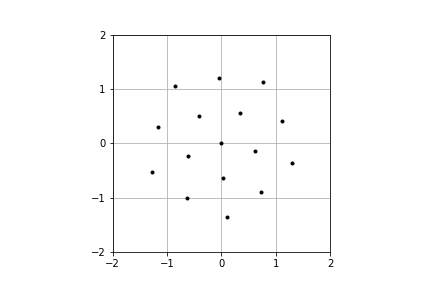
\includegraphics[width=\linewidth]{figures/leaky_relu_7_4_constellation_diagram.png}
       \caption{t-SNE dimension reduced constellation diagram for a (7,4) autoencoder model.}
   \end{subfigure}
   ~
   \begin{subfigure}[t]{0.3\textwidth}
       \centering
       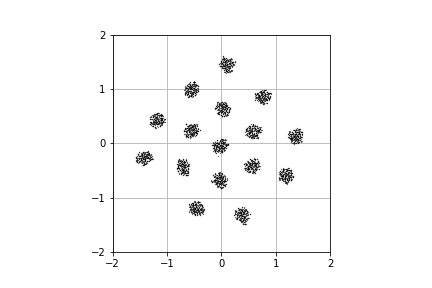
\includegraphics[width=\linewidth]{figures/tSNE_7_4_constellation_diagram_with_noise_200.png}
       \caption{200 full sets of all $M$ received symbols with noise.}
   \end{subfigure}
   \caption{t-SNE constellation diagrams}
   \label{fig:tSneConstellationDiags}
\end{figure*}

However some processing was required to produce the (7,4) tSNE constellation diagrams from ~\cite{oShea}'s Figures 4c and 4d. Firstly, despite the input to the tSNE function being normalised to have a constant unit instantaneous power constraint, the output has neither a non-zero power constraint, neither a zero mean. The constellation diagram was not at all stationary but an example of a typical constellation diagram is shown in Figure \ref{fig:tSneConstellationDiags}a.

Because of the lack of power constraint the output had to be manually scaled after the t-SNE processing. First the mean was set to zero, and then the signal was scaled to have an average power unit power. At this point a constellation diagram similar to ~\cite{oShea}'s Figure 4c was produced, an example is shown in Figure \ref{fig:tSneConstellationDiags}b. However it should also be noted that due to the t-SNE being a stochastic method, the constellation diagram changed every time. The central point is very rarely centred on zero and there are often less nice looking diagrams than Figure \ref{fig:tSneConstellationDiags}b. It is suggested that a perfect looking constellation diagram cannot be representative of a randomly selected iteration of the model.

Lastly a constellation diagram was produced of the channel symbols received at the transmitter from sending 200 of the full $M=16$ one-hot-encoded message sets through the AWGN channel. This constellation diagram is shown in Figure \ref{fig:tSneConstellationDiags}c. It was found that the small numbers of symbols transmitted with noise were much less likely to converge to a correct looking diagram, however increasing the number of symbols improved this somewhat, although not to the level of the constellations without noise like Figure \ref{fig:tSneConstellationDiags}b.

It is interesting that a (7,4) model with constant power constraint, once fed through t-SNE produces the same constellation diagram as ~\cite{oShea}'s Figure 4c did with a constant power constraint. This suggests that a similar process is performed by the t-SNE dimensionality reduction techinque. 

As the (7,4) model produced correct looking constellation diagrams, with the input to the t-SNE reduction being consistent an (8,8) model was produced and their BLER performances assessed. The initial performance of all the autoencoder models, with a relu model added for reference can be seen in Figure \ref{fig:AutoencodersAllOriginalComparison}.

\begin{figure}
   \centering
   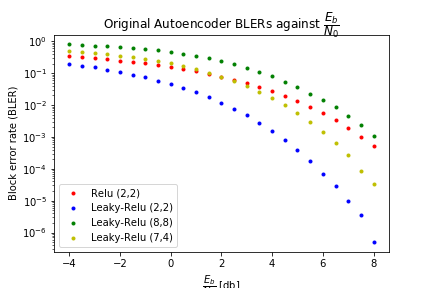
\includegraphics[width=0.6\linewidth]{figures/autoencoders248_bler_EbNo_original_comparison.png}
   \caption{Initial BLER performance comparison of (2,2), (8,8) and (7,4) autoencoder models. }
   \label{fig:AutoencodersAllOriginalComparison}
\end{figure}

The results from Figure \ref{fig:AutoencodersAllOriginalComparison} don't look correct. We expect the (7,4) autoencoder to have the best performance, followed by (8,8) and then a larger gap to (2,2). However in Figure \ref{fig:AutoencodersAllOriginalComparison} the (2,2) autoencoder is far and away the best of the models. Followed by the (7,4) autoencoder and then the (8,8) autoencoder. Also the (2,2) autoencoder model has a BLER $\approx10^2$ times lower than that achieved in ~\cite{oShea} accross the whole range of SNRs, which is suspicious. The (8,8) and (7,4) both significantly underperform in terms of BLER compared to those achieved in the paper. The only thing that does look correct is that \code{leaky-ReLu} outperforms \code{ReLu}. 

At this point the discovery that $Rr$ was not being set to the correct value mentioned in the two previous sections was made and applied to the leaky-ReLu models. The difference that this made can be seen in Figure \ref{fig:AutoencodersAllRr1Comparison}.

\begin{figure}
   \centering
   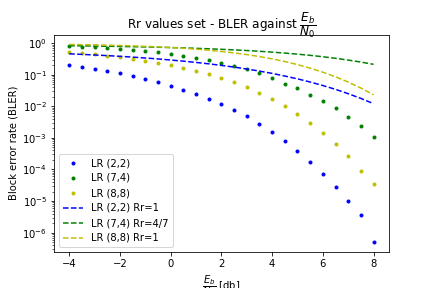
\includegraphics[width=0.6\linewidth]{figures/autoencoders248_bler_EbNo_Rr1_comparison.png}
   \caption{Comparison of BLER performance of (2,2), (8,8) and (7,4) autoencoder models before and after $Rr$ was set to the correct value. }
   \label{fig:AutoencodersAllRr1Comparison}
\end{figure}

The results after setting the $Rr$ correctly look just as incorrect as the results that preceded them, although differently. Before, the (2,2) autoencoder outperformed the results in the paper, now all three models clearly significantly underperform the results in the paper. The relative ordering is still wrong in the same way, although the shape of the (8,8) autoencoder's BLER looked more promising. This was because it started off with poor performance and then showed strong improvement over the high SNRs, which was what was found in ~\cite{oShea}'s Figure 3b.

At the end of this section the (7,4) and (8,8) autoencoder models are clearly significantly underperforming. This was seen as a problem and so was addressed in the section after next (Section\ref{sec:Improving88And74}). However it was noticed that, apart from in extreme cases, it was hard to tell if the (7,4) model was overperforming or underperforming. In ~\cite{oShea} the (7,4) autoencoder produced indistinguishable performance from the Hamming (7,4) MLD method. So the next section focussed on producing Hamming (7,4) MLD, in order to be able to better assess performance of the (7,4) model.

\subsubsection{Finding errors and improving performance}

\label{sec:Improving88And74}

At this point all of the models had been implemented, so the focus of this section was to find any bugs and improve the models to give equal or better performance to those in the paper. The ordering of the models was the opposite of what would be expected. From best to worst the ordering was (2,2), (7,4) then (8,8), whereas it would be expected (7,4), (8,8) then (2,2). Additionally BPSK was significantly overperforming.  

The first place to start was that the (7,4) and (8,8) models were significantly underperforming. It was thought that the more complex models might be underperforming from underfitting due to insufficient layers or an unsuitable activation function. At this point the activation function of all the layers other than the final receiver layer had a \code{leaky-ReLu} activation function. It was also thought that the layer widths dropping in one step from 256 to 8 for the (8,8) case may be causing the issue. So a general function was written to produce an $n$ layer model, with the last layer having a \code{tanh} activation function to capture non-linearity. This model also had linearly tapered layer widths to try and improve the fitting of the function. 

In the development of the generalised $n$ layer model it was found that due to a bug in the \code{make$\_$model} function the (8,8) model was actually implementing an (8,4) model. Retifying this error instantaneously improved the validation loss during training at an $\frac{E_b}{N_0} = 7db$ from 1.06 to 0.0750. The performance of the different layered models with the (8,4) bug corrected can be seen in Figure \ref{fig:NumLayersBler}.

\begin{figure}[t]
   \centering
   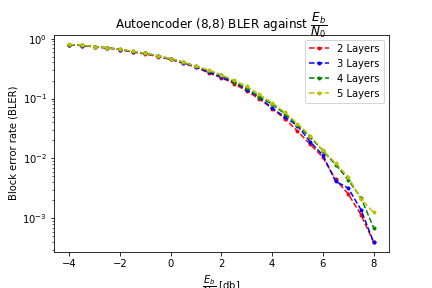
\includegraphics[width=\genfigsize\linewidth]{figures/autoencoder_8_8_bler_EbNo_2-5_layers.png}
   \caption{Comparison of different number of layers for the (8,8) autoencoder model.}
   \label{fig:NumLayersBler}
\end{figure}


The four and five layer models were seperably worse, and the two layer model very marginally outperformed the three layer model, however the margin negligible. In machine learning it is customary to increase the complexity of the model, and pick the complexity at which the training error stopped significantly improving to avoid overfitting.

However as in this project the data is synthetically generated, exceptionally uniform, the noise is newly generated for each transmission and the data sets used for training and testing are very large there is not much worry of overfitting.

So where normally decisions on hyperparameters would only be made based on performance over the validation set, in this project decisions have consistently been made based on performance on the test set. This section is no different. 

Two layers was selected as the number of layers, because it had the best (although very marginally) performance over the test set. Additionally it was the simplest model complexity wise and so trained more quickly and was less likely to overfit.

Due to the indistinguishable performance of the last layer being a \code{tanh} activation function it was left in as it had a good theoretical backing. The \code{tanh} function exhibits linear like behaviour for small values, but can also introduce non-linearity, which the \code{leaky-ReLu} function could not.

After the discovery of the (8,4) bug and the confirmation that the number of layers and lack of non-linearity was not the issue with the (8,8) model, the (8,8) autoencoder was performing better, but still not well enough. 

\subsubsection{Finding incorrect scaling}
\label{sec:CorrectingScaling}

The continued lack of performance and easy find of the (8,4) bug led to the (7,4) model being investigated instead. It was realised that the models were being unfairly normalised. All the complex models were being normalised such that each complex channel symbol had an instantaneous power of 1. However the (7,4) model was being normalised such that each (7,1) channel encoded message had an instantaneous power of 1. This meant an average power of $\frac{1}{7}$ for each channel bit, whereas the complex (2,2) and (8,8) models had an average power of $\frac{1}{2}$ per channel bit. Going further it was realised that this was again unfair when compared to BPSK, which had a power of 1 per bit. 

Due to uncertainty about what the correct average power per channel bit should be a meeting was aranged with the co-supervisor who confirmed that there should be an average power of 1 per channel bit. So a total power of $n_r$ per channel message. 

To solve this problem a scaling layer was added after the normalisation layer. The normalisation layer normalised the last axis of the transmitter tensor to have and L2-norm (power) of 1. The following layer then multiplied the channel symbols by a factor of $\sqrt(N_r)$ to give a message power of $N_r$. 

In order to get the correct results for all models quickly, training of the models and running of the performance cells was switched to an AWS instance. The instance used was a g3.4xlarge, the hardware details of which are described in Section \ref{sec:HardwareAnalysis}. This model has a GPU and 16 CPU cores. This resulted in training models approximately fifteen times faster and allowed the performance loops to be effectively parallelised with a speedup of approximately ten times. 

\begin{figure}[t]
   \centering
   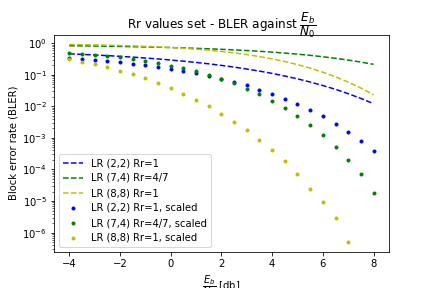
\includegraphics[width=\genfigsize\linewidth]{figures/autoencoders_correct_scaling_comparison.png}
   \caption{Comparison of performance of all autoencoder models before and after introducing correct scaling.}
   \label{fig:AutoencodersAllScalingComp}
\end{figure}

The improvements of performance from introducing correct scaling of the channel symbols can be see in Figure \ref{fig:AutoencodersAllScalingComp}. The results show that the larger models were being unfairly penalised as the (2,2) autoencoder marginally improves, whereas the (7,4) and (8,8) models both significantly improve by factors of $\approx 10^5$ at the high SNRs. 

The (8,8) model worked first time, however the (7,4) took a little longer to get working as there was a bug where the scaling layer was being skipped.

After this correction the (7,4) model performs more or less inline with what it should according to ~\cite{oShea}, as does the (2,2) model. However the (8,8) model far outperforms it's counterpart from ~\cite{oShea}. In fact the (8,8) model had to be rerun on the AWS instance with larger data set to give a smooth curve at such low error rates. 

At this point the next iteration of ~\cite{oShea}'s Figure 3a and 3b were plotted. The results can be seen in Figure \ref{fig:OSheaFig3Incorrect88}.

\begin{figure*}[t!]
   \centering
  \begin{subfigure}[t]{0.45\textwidth}
       \centering
       
\includegraphics[width=\linewidth]{figures/o_shea_3a_bler_vs_eb.png}
       \caption{Final reproduction of ~\cite{oShea}'s Figure 3a, before adding BCH codes and redebugging Hamming HD.}
       \label{fig:OSheaFigure3aIncorrect88}
   \end{subfigure}
   ~
   \begin{subfigure}[t]{0.45\textwidth}
       \centering
       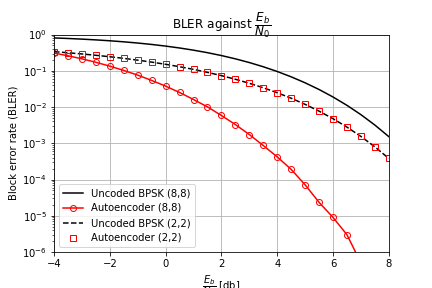
\includegraphics[width=\linewidth]{figures/o_shea_3b_bler_vs_eb_88_scaled_incorrectly.png}
       \caption{Penultimate reproduction of 3b, with overperforming (8,8) model due to incorrect scaling.}
       \label{fig:OSheaFigure3bIncorrect88}
   \end{subfigure}
   \caption{t-SNE constellation diagrams}
   \label{fig:OSheaFig3Incorrect88}
\end{figure*}

\subsubsection{Final corrections and BCH coding}

At this point after submitting a draft of the first two sections of the report to the supervisors the returning advice was to compare the performance against BCH codes instead. Consequently BCH codes will be investigated later in this section.

The current differences between ~\cite{oShea}'s Figure 3a and 3b, comared to Figure \ref{fig:OSheaFig3Incorrect88}a and b are that the (8,8) model significantly overperforms and the Hamming (7,4) HD significantly underperforms. The first of these to be investigated was the (8,8) autoencoder. 

It was noticed while writing up Section \ref{sec:CorrectingScaling} that the reason for this was the scaling being incorrectly applied to the (8,8) complex model. As the L2-normalisation is applied to the last dimension, the same method cannot be applied to the (7,4) non-complex and (8,8) complex models. 

The (7,4) model's channel symbols must be multiplied by a factor of $\sqrt{N_r}$ because the last dimension is the (7,) dimension. However the last dimension in the complex model is the complexity dimension of shape (2,). So the channel symbols must be scaled by a factor of $\sqrt{2}$. This means that the performance of the (2,2) model is correct by chance, however the symbols of the (8,8) model are being scaled up incorrectly by an extra factor of 2.

This was rectified giving the performance shown in Figure \ref{fig:Autoencoders88ScalingCorrected}.

\begin{figure}[t]
   \centering
   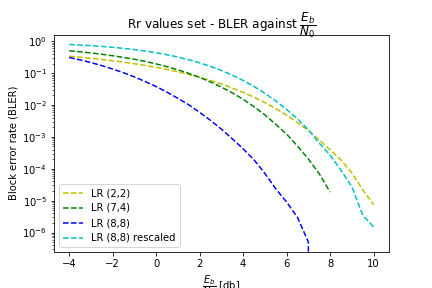
\includegraphics[width=\genfigsize\linewidth]{figures/autoencoders_recorrected_88_scaling.png}
   \caption{Comparison of performance of all autoencoder models after (8,8)s scaling was corrected.}
   \label{fig:Autoencoders88ScalingCorrected}
\end{figure}

\begin{figure*}[t!]
   \centering
  \begin{subfigure}[t]{0.45\textwidth}
       \centering
       \includegraphics[width=\linewidth]{figures/o_shea_3a_bler_vs_eb.png}
       \caption{Final reproduction of ~\cite{oShea}'s Figure 3a, before adding BCH codes and redebugging Hamming HD.}
       \label{fig:OSheaFigure3a}
   \end{subfigure}
   ~
   \begin{subfigure}[t]{0.45\textwidth}
       \centering
       \includegraphics[width=\linewidth]{figures/o_shea_3b_bler_vs_eb.png}
       \caption{Final reproduction of 3b, three lines identical, (8,8) autoencoder slightly underperforming.}
       \label{fig:OSheaFigure3b}
   \end{subfigure}
   \caption{t-SNE constellation diagrams}
   \label{fig:OSheaFig3}
\end{figure*}

After correcting the incorrect scaling of the (8,8) autoencoder to a factor of $\sqrt{2}$ the results graph looks as it does in Figure ~\cite{fig:OSheaFigure3b}. This is now very similar to Figure 3a from ~\cite{oShea}. Three of the lines are identical, the (2,2) autoencoder and both the BPSK models. The (8,8) autoencoder line is similar in that it starts in tangent with the (8,8) BPSK and finishes with the lowest error rate. However it slightly underperforms it's counterpart from ~\cite{oShea}. It crosses the (2,2) lines at $\approx7$ as opposed to $\approx5.5$. The BLER seems to be roughly a factor of 5 out. This suggests there may be some small change to the architecture that can be made to improve performance. However the number of layers and activation functions have already been varied. One option left is dropout regularisation. This is where some fraction of the neurons are switched off randomly at training time, which is done primarily to avoid overfitting. However this hasn't been trialed so far because the data sets are very uniform, very large, and the noise is newly randomly generated every time the model transmits a message. Because of this it seems unlikely that the model could overfit. 

Additionally the (7,4) autoencoder in Figure \ref{fig:OSheaFigure3a} is also slightly underperforming at the high SNRs. As this margin is so small it will be tackled by retraining and using the ModelCheckpoint callback to ensure that the model with the best validation loss achieved during the training process is saved. Also the model will be retrained over a large number of initialisations to remove any small dependence on initialisation values. This has not been used before due to the very large time commitment that is needed for training a large number of models fully. 

The last inconsistency in Figure \ref{fig:OSheaFig3} is that the Hamming HD encoding is significantly underperforming. A reasonable amount of time has been committed to debugging this and the underlying BPSK, however it seems to perform correctly in all unit tests and have the correct amount of noise being applied so the author can not see what is being implemented incorrectly. 


BCH codes were investigated on the direction of a project supervisor. BCH codes are a generalisation of Hamming codes for multiple error corrections, where the number of errors which can be corrected is specified as a variable design parameter $t$. For any integers $m \geq 3$ and $t < 2^{m-1}$ there exists a BCH code with the characteristics described in Equations \ref{eq:BchCharacteristics} where $k$ is the number of data bits. Note that the minimum distance is ofter referred to as the designed distance.

\begin{align}
   \mbox{block length: }& n = 2^{m}-1 \nonumber\\
   \mbox{parity bits: }& n-k\leq mt \nonumber\\
   \mbox{minimum distance: }& d_{min} \geq 2t+1
   \label{eq:BchCharacteristics}
\end{align}

The (7,4) Hamming code examined above is a special case of the BCH code where $m=3$ and $t=1$. It would have been interesting to look at the next BCH code up where $k=4$ and $t=2$, or in the same ratio. The \code{python-bchlib} library~\cite{BchGithub} written by J.Kent was used for encoding and decoding. It seemed a good idea to start with the $m=3$ and $t=1$ case as it is the same as Hamming (7,4) so the results should be easily comparible.

\begin{figure}
   \centering
   \includegraphics[width=\genfigsize\linewidth]{figures/gaussian_pdf.png}
   \caption{Gaussian pdf for illustration.}
   \label{fig:GaussianPdf}
\end{figure}

The implementation code for this section can be found in the \textit{BCH$\ $Encoding} section of \code{initial$\_$dnn$\_$comms.ipynb}. It required a seperate noise generation section function as the \code{bchlib} encoding functions output bytearrays instead of numpy arrays.  The noise function is called \code{gaussian$\_$bitflip}, It works on the basis that the noise is AWGN distributed, so has the pdf shown in Figure \ref{fig:GaussianPdf}. The red highlighted area from Figure \ref{fig:GaussianPdf} represents the probability of error for a transmitter BPSK signal. The \code{gaussian$\_$bitflip} function takes in normal binary encoded signals and assumes that they would have been encoded into BPSK and then passed through an AWGN channel. So $p_e$ is given by Equation ref{eq:GaussianBitflip}.

\begin{align}
   p_e =& P(X \leq -1) \nonumber\\
   =& CDF(-1)
   \label{eq:GaussianBitflip}
\end{align}

So the function goes through every bit sent, and with probability $p_e$ flips the bit by XORing (exclusive or'ing) with 1 $<<$ bit$\_$number, which is the number one logically shifted left by bit$\_$number bits. This function therefore directly replicates the effect of encoding into BPSK, adding gaussian noise, picking the most likely symbol and decoding back to binary. Using this function the two lines in Figure \ref{fig:BchT1VsT2} were produced to compare the BLER of a BCH code with $t=1$ and $t=2$. 

\begin{figure*}[t!]
   \centering
  \begin{subfigure}[t]{0.45\textwidth}
       \centering
       \includegraphics[width=\linewidth]{figures/bch_t1_vs_t2.png}
       \caption{A figure to show the performance of two BCH codes with $t=1$ and $t=2$ respectively.}
       \label{fig:BchT1VsT2}
   \end{subfigure}
   ~
   \begin{subfigure}[t]{0.45\textwidth}
       \centering
       \includegraphics[width=\linewidth]{figures/o_shea_3a_bler_vs_eb_bch.png}
       \caption{The reporduction of ~\cite{oShea}'s Figure 3a with BCH encoding added for extra comparison.}
       \label{fig:OSheaFigure3aBch}
   \end{subfigure}
   \caption{t-SNE constellation diagrams}
   \label{fig:BchFigures}
\end{figure*}

As expected the $t=2$ line outperforms the $t=1$ line. Although as mentioned above the $t=1$ line should give identical performance to the Hamming (7,4) line. As mentioned earlier the Hamming (7,4) line in Figure \ref{fig:OSheaFig3} underperforms. 

IF THE RESULTS LOOK GOOD THEN I COULD USE BCH1 INSTEAD OF HAMMING (7,4) AS MY HAMMING (7,4) LINE.

CONVERT TO THIS COULD BE IMPLEMENTED WITH MORE INFORMATION IF IMPLEMENTED IN MATLAB ETC.

Unfortunately the results from this method and library were not at all satisfactory. The BLER for the above case are shown in Figure \ref{fig:BchT1VsT2}. Sadly as this was investigated in response to feedback and so the implementation was done just a couple of days before the report was due there was not enough time to properly debug this section. The results are clearly wrong in that the BLER converges to $\approx0.2445$ at very high SNRs. The suspected reasons for this are that the BCH polynomial prime used (8129) is unsuitable or  

It was suggested in a second meeting that this could be easily implemented in Matlab, however as the rest of the project was already implemented in python, the author wasn't recently familiar with Matlab and the deadline was the following day there was not enough time to investigate this option. 

\subsection{Paper 2 - Reinforcement learning, RBF and RF}

\begin{itemize}
   \item Introduction to Rayleigh
   \item Description of architecture of models in the paper
   \item Rayleigh slow fading model and results
   \item Rayleigh block fading attempt 
\end{itemize}

\subsection{Rayleigh Fading}

Rayleigh fading is a type of fading which models a channel in which there is not a clearl line of sight between the receiver and the transmitter, this is a good approximation for signal propogation through the troposhpere and ionoshpere as well as built up areas like cites~\cite{RayleighProakis}. The fading implemented in this report is assumed to be flat and slow. The large and small scale fading are assumed to be stationary. Rayleigh fading is implemented by the equation below.

\begin{align}
   \mathbf{r} = \mathbf{s}*\mathbf{h} + \mathbf{n} \mbox{ }&\nonumber\\
   \mbox{where:}\mathbf{h} &= h_r + jh_i \nonumber\\
   \mathbf{n} &= n_r + jn_i \nonumber\\
   n_r,n_i &\sim \mathcal{N}(0,\sigma_a^2) \nonumber\\
   h_r,h_i &\sim \mathcal{N}(0,\sigma_m^2) \nonumber\\
   \label{eq:RaylieghDef}
\end{align}

$\mathbf{s}$ and $\mathbf{r}$ are the complex sent and received signals respectively. In all types of rayleigh fading a different realisation of $n$ is used for every sent signal, but the same does not apply to $h$. In RBF (rayleigh block fading) the multiplicative factor $h$ stays the same for the whole block of sent messages. In rayleigh slow fading (RSF) h changes every message that is sent but remains the same for each bit of the message, whereas rayleigh fast fading (RFF) would have both $h$ and $n$ changing during the sending of each symbol, so each symbol would be transmitter over multiple fades. The Aoudia paper examined RBF.



\subsubsection{Investigation into RSF}

The first objective was to reproduce the supervised AWGN graph from ~\cite{Aoudia}. This was very easily done by simply using the (8,8) model from the previous section to produce Figure \ref{fig:AwgnSupervised}.

\begin{figure}
   \centering
   \includegraphics[width=\genfigsize\linewidth]{figures/aoudia_paper/awgn_supervised.png}
   \caption{Reproduction of ~\cite{Aoudia}'s Figure 6a, only supervised line currently present.}
   \label{fig:AwgnSupervised}
\end{figure}

COMMENT ON WHETHER THIS LINE LOOKS LIKE THE ONE IN THE PAPER.

After producing the supervised AWGN model it was decided to investigate RSF before RBF. This was because they required very similar noise layers, but the RSF model would have a significantly simpler architecture. This architecture can be seen in Figure \ref{fig:RsfSupervisedArch}. The architectures of the individual blocks can be seen in Figure \ref{fig:RsfArchitectures}

\begin{figure}
   \centering
   \includegraphics[width=\genfigsize\linewidth]{figures/aoudia_paper/autoencoder_rsf_arch.png}
   \caption{The architecture of the whole end-to-end system of }
   \label{fig:RsfSupervisedArch}
\end{figure}

\begin{figure*}[t!]
   \centering
  \begin{subfigure}[t]{0.3\textwidth}
       \centering
       \includegraphics[width=\linewidth]{figures/aoudia_paper/transmitter_rsf_arch.png}
       \caption{A block diagram of the RSF transmitter architecture.}
       \label{fig:RsfTxArch}
   \end{subfigure}
   ~
   \begin{subfigure}[t]{0.3\textwidth}
       \centering
       \includegraphics[width=\linewidth]{figures/aoudia_paper/h_estimator_rsf_arch.png}
       \caption{A block diagram of the RSF $\hat{h}$ estimator architecture.}
       \label{fig:RsfHestArch}
   \end{subfigure}
   ~
   \begin{subfigure}[t]{0.3\textwidth}
       \centering
       \includegraphics[width=\linewidth]{figures/aoudia_paper/receiver_rsf_arch.png}
       \caption{A block diagram of the RSF receiver architecture.}
       \label{fig:RsfRxArch}
   \end{subfigure}
   \caption{Block diagrams showing the architectures of all the submodels of the RSF autoencoder model shown in Figure \ref{fig:RsfSupervisedArch}.}
   \label{fig:RsfArchitectures}
\end{figure*}

These architectures show the addition of an expert feature as an advancement from the AWGN supervised models. This is the \code{HEstimator} section, which makes an estimate of the $\mathbf{h}$ parameter from Equation \ref{eq:RaylieghDef} for that message. There is then a \code{y$\_$over$\_$h} layer which implements complex division of the received signal by the output of the \code{HEstimator}. Note that the received signal has shape (batch$\_$size,$N_c$,2) and estimated h has shape (batch$\_$size,2). So a $\hat{h}$ is found for each overall message which is sent, and then all four of the transmitter complex channel symbols are divided by this factor. 

The transmitter architecture has also changed 

The receiver architecture has changed 

The h-estimator layer structure is taken from the architecture in the paper.


\subsubsection{Investigation into RBF}



\FloatBarrier
\section{Results}

\begin{itemize}
   \item I mainly produced the same results as them.
   \item 
\end{itemize}


\FloatBarrier
\section{Evaluation}

\begin{itemize}
   \item Learned model performed very poorly on Rayleigh Slow Fading, it is likely it would perform even more poorly on Rayleigh Fast Fading.
\end{itemize}

\FloatBarrier
\section{Conclusions}

\begin{itemize}
   \item I couldn't replicate their performance with their architectures. I found that they underperformed their results.
   \item This method is unlikely to produce results from Rayleigh Fast Fading channels, potentially RNNs would be better there as they could maybe learn waterfilling?
   \item 
\end{itemize}


\FloatBarrier
\section{Future Work}

REWORD THIS STUFF INTO FUTURE WORK

\textit{
Some extra comparisons which will be completed if there is time to check that the developed methods are truly competitive with state of the art are comparing the learned systems to Shannon's theoretical capacity limit and current state of the art codes such as turbo and LDPC codes for an AWGN channel.
}

\textit{
Another additional comparison which may be done if there is time is to compare the learned networks and current state of the art across common fading channels such as Rayleigh and Ricean channels across a range of type of fading, large scale or small scale, fast or slow, flat or frequency selective. This would better assess the generality of a learned communction system than has so far been done in the literature.
}

\textit{
After which ideally the same could be done for some rare or hard to model channels. These being where the learned communication system should have the biggest advantage and so it would be interesting to see if they could deliver on their potential.
}

\textit{
If the main deliverables are finished then further research will be started by investigating adding an RTN layer to the receiver of the reinforcement learning model. The project supervisor had stated that
if section is reached then he will decide which of the two areas is most current between reinforcement learning and SWIPT and further research will be continued into this area. The details of these deliverables are described in the project specification, however as these will be new areas a different method of evaluating the success and validity of the results.
}

\begin{itemize}
   \item Remember that slow fading with short block lengths was a potentially advantageous environment for learned communication systems
   \item Also cities with very complicated environments, lots of multipaths, no direct lines of sight, stationary and significant large scale would be an environment where the learned communication system would likely do well.
   \item Look at the "Types of fading" section for more details.
\end{itemize}


\FloatBarrier
\appendix
\section{Appendix}

\section{Ethical, Legal and Safety Considerations}

\subsection{Ethical considerations}

One interesting ethical consequence of this project is that, if this technology were to become very successful and so very competitive with or superior to current state of the art communications systems, it could reduce the number of jobs for communications engineers. If it was possible to just set up a generic transmitter and receiver, then let them train for their environment and then just have them run at optimal performance, there there would not be as much of a need for communications engineers to design systems.

While this would be bad for current communications engineers, it would lead to greater productivity and efficiency by companies which would contribute to greater economic growth, which would then trickle back down. So while it may be bad for a minority, it should be better for the majority, therefore overall it is ethically alright. However other than this there are no significant ethical implications of this project.

\subsection{Legal consideration}

\subsubsection{Infringing patents}

A search was performed on Espacenet, which was found by direction from the UK government website. This seach of Espacenet was to see if there were any parents which this project might be infringing. Patents were searched for using related key words, however no patents of similar ideas were found. Consequently the project is likely safe from infringing any patents. If there were any significant commercial consequences of this report then a more thorough search could be carried out through a patent attorney, however this would be expensive and is unlikely to be needed.

The legal alternative to patents for protection of intellectual property is referred to as a "trade secret". However these are only legally binding for company employees who have signed a non disclosure agreement (NDA), or if someone is accessing the information either when they do not have the permission to access it, or they are receiving it from someone who doesn't have the permission to access it. Trade secrets become non-binding once the information is publicly available, so as the papers that this paper is reproducing are publicly available it cannot be infringing any trade secrets that the author is unaware of. 

\subsubsection{Use of data}

The other potential legal concern for a project of this type is potentially using someone's data inappropriately while training a machine learning model. For the first part of this project this isn't possible as the model involves training an autoencoder-like model. In this method the desired output is the initial input, and that input is any one of the potential combinations of n binary bits. This is where n is the block length. Hence there is no involvement of non-self-generated data and so can be no illegal use of someone else's data.

In the last of the main deliverables where would be developing the reinforcement learning model which could be trained on any samples from any channel there is marginally more of a risk of this. To counter this risk it will be made sure that these samples are sourced from publicly available sources, so people who have contributed to it will have signed that they consented to having their data collected. 

However it should be made clear that it should be more or less impossible to decode the information that people were sending across a channel from the channel interference samples. To ensure there can be no accusations of this the data and model will be kept private, results will not be shared publicly and there will be no inspection of the channel interference.

\subsubsection{Licences of used libraries}

The Keras library has an MIT lisence, which means that users have the right to "use, copy, modify, merge, publish, distribute, sublicense, and/or sell copies of the Software" as long as a copyright notice is place in the code. To ensure that this is abided by, if the software from this project is published then Keras will be acknowledged and referenced. Additionally the copyright stamp will be included in the code if it is published. 

\subsection{Safety Plan}

Firstly it should be stated that compared to hardware projects there are no really pressing safety issues. However the relevant safety issues are assessed in Table \ref{tab:RiskAssessment}. 

\begin{table*}[!htbp]
\resizebox{\textwidth}{!}{
\centering
{\small \hfill{}
\small
\begin{tabular}{|p{1.2cm}|p{1.5cm}|p{1.3cm}|p{1.2cm}|p{7cm}|}
\hline
\textbf{Risk}                  & \textbf{Potential Cause}          & \textbf{Likelihood (/5)} & \textbf{Potential Harm (/5)} & \textbf{Mitigation Plan}                                                                                                                                                                                                                                                       \\ \hline
Repetitive strain injury (RSI) & Excessive use of laptop           & 4                        & 1                           & I will take regular breaks every 20-60 minutes. If I get RSI then I will identify what movement is causing it and stop this movement. I will also treat it with hot and cold treatment, rest and anti-inflammatories like ibuprofen.  {[}{]}                                    \\ \hline
Eye Strain                     & Excessive use of laptop           & 4                        & 2                           & To avoid straining my eyes I will try to work with adequate, but not too bright, lighting at all times, and will rest my eyes every twenty minutes. I will also try to keep the screen approximately 20-24 inches away from my eyes and 10-15 inches below my eye line. {[}{]} \\ \hline
Back Pain                      & User's poor posture               & 2                        & 2                           & I have set my chair at my work station up according to this NHS guide {[}{]} and a will make more effort to sit with correct posture to avoid back pain which might prevent me from working.                                                                                   \\ \hline
Trip Hazards                  & Often work with laptop plugged in & 1                        & 2                           & I will make sure that my charger lead is as short as possible and does not stretch across any areas where people regularly walk.                                                                                                                                               \\ \hline
Electric shocks                & Often work with laptop plugged in & 1                        & 5                           & I will be careful when plugging and unplugging my laptop to avoid shocking myself.                                                                                                                                                                                             \\ \hline
Fires                          & Often work with laptop plugged in & 1                        & 5                           & I will not leave my laptop plugged in unsupervised. I have also checked that my laptop charger has been PAT tested and so I think I have taken reasonable steps.                                                                                                               \\ \hline
\end{tabular}
}}
\caption{Risk assessment in table form}
\label{tab:RiskAssessment}
\end{table*}


{\small
\bibliographystyle{ieeetr}
\bibliography{egbib}
}

\end{document}
